%%%%%%%%%%%%%%%%%%%%%%%%%%%%%%%%%%%%%%%%%%  不使用 authblk 包制作标题  %%%%%%%%%%%%%%%%%%%%%%%%%%%%%%%%%%%%%%%%%%%%%%
%-------------------------------PPT Title-------------------------------------
\title{材料模拟软件与方法简介\rm{(I)}}
%-----------------------------------------------------------------------------

%----------------------------Author & Date------------------------------------
%\author[\textrm{Jun\_Jiang}]{姜\;\;骏\inst{}} %[]{} (optional, use only with lots of authors)
%% - Give the names in the same order as the appear in the paper.
%% - Use the \inst{?} command only if the authors have different
%%   affiliation.
\institute[BCC]{\inst{}%
%\institute[Gain~Strong]{\inst{}%
\vskip -20pt 北京市计算中心~云平台事业部~姜骏}
%\vskip -20pt {\large 格致斯创~科技}}
\date[\today] % (optional, should be abbreviation of conference name)
{	{\fontsize{6.2pt}{4.2pt}\selectfont{\textcolor{blue}{E-mail:~}\url{jiangjun@bcc.ac.cn}}}
\vskip 45 pt {\fontsize{8.2pt}{6.2pt}\selectfont{北京科技大学% 报告地点
	\vskip 5 pt \textrm{2024.03.28}}}
}

%% - Either use conference name or its abbreviation
%% - Not really information to the audience, more for people (including
%%   yourself) who are reading the slides onlin%%   yourself) who are reading the slides onlin%%   yourself) who are reading the slides onlineee
%%%%%%%%%%%%%%%%%%%%%%%%%%%%%%%%%%%%%%%%%%%%%%%%%%%%%%%%%%%%%%%%%%%%%%%%%%%%%%%%%%%%%%%%%%%%%%%%%%%%%%%%%%%%%%%%%%%%%

\subject{}
% This is only inserted into the PDF information catalog. Can be left
% out.
%\maketitle
\frame
{
%	\frametitle{\fontsize{9.5pt}{5.2pt}\selectfont{\textcolor{orange}{“高通量并发式材料计算算法与软件”年度检查}}}
\titlepage
}
%-----------------------------------------------------------------------------

%------------------------------------------------------------------------------列出全文 outline ---------------------------------------------------------------------------------
\section*{}
\frame[allowframebreaks]
{
  \frametitle{Outline}
%  \frametitle{\textcolor{mycolor}{\secname}}
  \tableofcontents%[current,currentsection,currentsubsection]
}
%%在每个section之前列出全部Outline
%%类似的在每个subsection之前列出全部Outline是\AtBeginSubsection[]
%\AtBeginSection[]
%{
%  \frame<handout:0>%[allowframebreaks]
%  {
%    \frametitle{Outline}
%%全部Outline中,本部分加亮
%    \tableofcontents[current,currentsection]
%  }
%}

%-----------------------------------------------PPT main Body------------------------------------------------------------------------------------
\small
%\section{引言}
\frame
{
	\frametitle{\rm{I~Have~A~Dream}}
\begin{figure}[h!]
\vspace*{-0.18in}
\centering
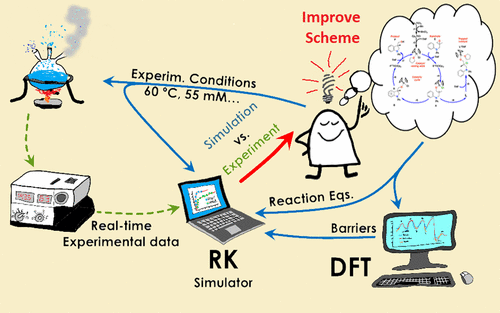
\includegraphics[height=2.55in,width=4.05in]{Figures/Schematic_Material-Design.png}
%\caption{\tiny \textrm{Pseudopotential for metallic sodium, based on the empty core model and screened by the Thomas-Fermi dielectric function.}}%(与文献\cite{EPJB33-47_2003}图1对比)
%\caption{\tiny \textrm{Pseudopotential for metallic sodium, based on the empty core model and screened by the Thomas-Fermi dielectric function.}}%(与文献\cite{EPJB33-47_2003}图1对比)
\label{Schematic_Material-Design}
\end{figure}
}


\frame
{
	\frametitle{材料模拟的基本思想和方法}
\begin{figure}[h!]
\vspace*{-0.25in}
\centering
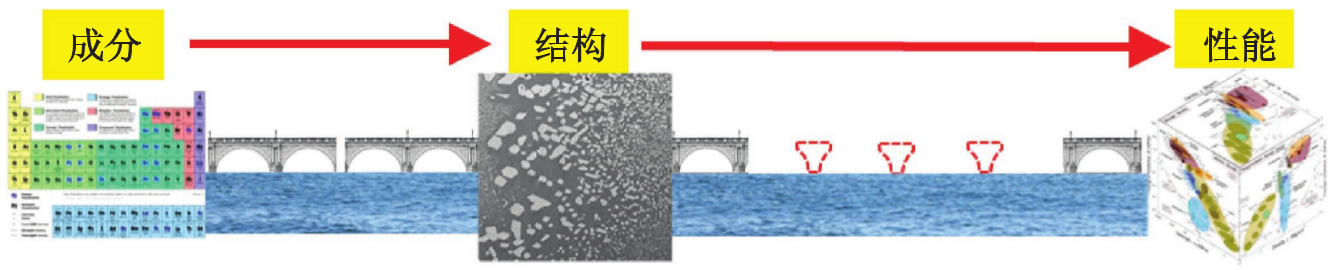
\includegraphics[height=0.80in,width=4.05in]{Figures/MGE-2.png}
%\caption{\tiny \textrm{Pseudopotential for metallic sodium, based on the empty core model and screened by the Thomas-Fermi dielectric function.}}%(与文献\cite{EPJB33-47_2003}图1对比)
\vskip 0.05pt
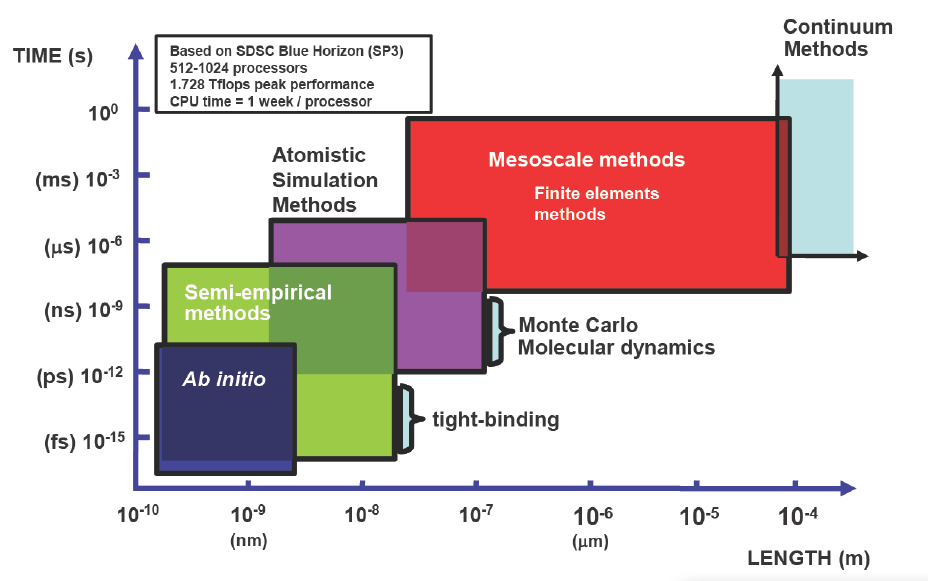
\includegraphics[height=2.20in,width=3.45in]{Figures/Multi-Scale-6.png}
%\caption{\tiny \textrm{Pseudopotential for metallic sodium, based on the empty core model and screened by the Thomas-Fermi dielectric function.}}%(与文献\cite{EPJB33-47_2003}图1对比)
\label{Multi-Scale}
\end{figure}
}

\frame
{
%	\frametitle{\textrm{DFT-SCF}}
\begin{figure}[h!]
\vspace*{-0.25in}
\centering
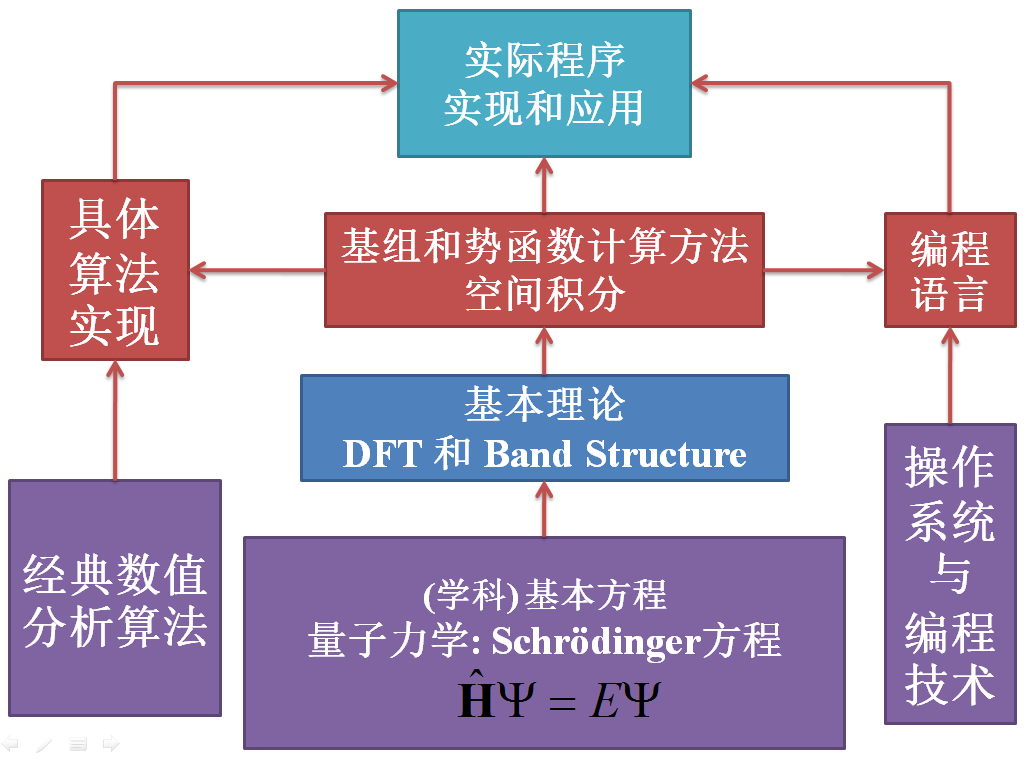
\includegraphics[height=2.80in,width=4.95in,viewport=5 3 1250 780,clip]{Figures/Method_Procedure.png}
%\caption{\tiny \textrm{Pseudopotential for metallic sodium, based on the empty core model and screened by the Thomas-Fermi dielectric function.}}%(与文献\cite{EPJB33-47_2003}图1对比)
\label{Method-Procedure}
\end{figure}
}

%-----------------------------------------------------------------------------------------------------------------------------------------------------------------------%
\section{从理论到计算软件:~以\rm{DFT}为例}       %Bookmark
\subsection{密度泛函理论}       %Bookmark
\frame
{
	\frametitle{\textit{ab~initio}和\textrm{first~principle}}
	\begin{itemize}
		\item \textit{ab~initio}是拉丁文词汇\textrm{(Latin~term)},其含义是\textrm{``from the beginning''},由拉丁文\textit{ab}~\textrm{(``from'')}+\textit{initio}~\textrm{(``beginning'')}合成,后者是\textit{initium}的单数夺格\footnote{\fontsize{5.5pt}{4.2pt}\selectfont{夺格\textrm{(ablative)},又称离格或从格,语法功能上表示某些词汇的状语。拉丁文\textit{initium}的意思是''开始、初始''。}}
		\item \textit{ab~initio}常用于法律和科学领域,如从头计算法(\textit{ab~initio}~\textrm{method})。法律中,\textit{ab~initio}表示"一开始即如此,而非法院宣判之后"。
		\item \textrm{first~principle}指从基本的物理学定律出发,不外加假设与经验拟合的推导与计算。
		\item 在物理学领域,\textrm{first~principle}(第一性原理)和\textit{ab~initio}(从头计算)含义上是等价的。例如利用\textrm{Schr\"odinger}方程在一些近似条件下求解电子结构,但无须依赖实验数据得到拟合参数的方法,就是第一原理或从头计算法。
	\end{itemize}
}

\frame
{
	\frametitle{\textit{ab~initio} \textrm{in inscription}}
\begin{figure}[h!]
\vspace*{-0.15in}
\centering
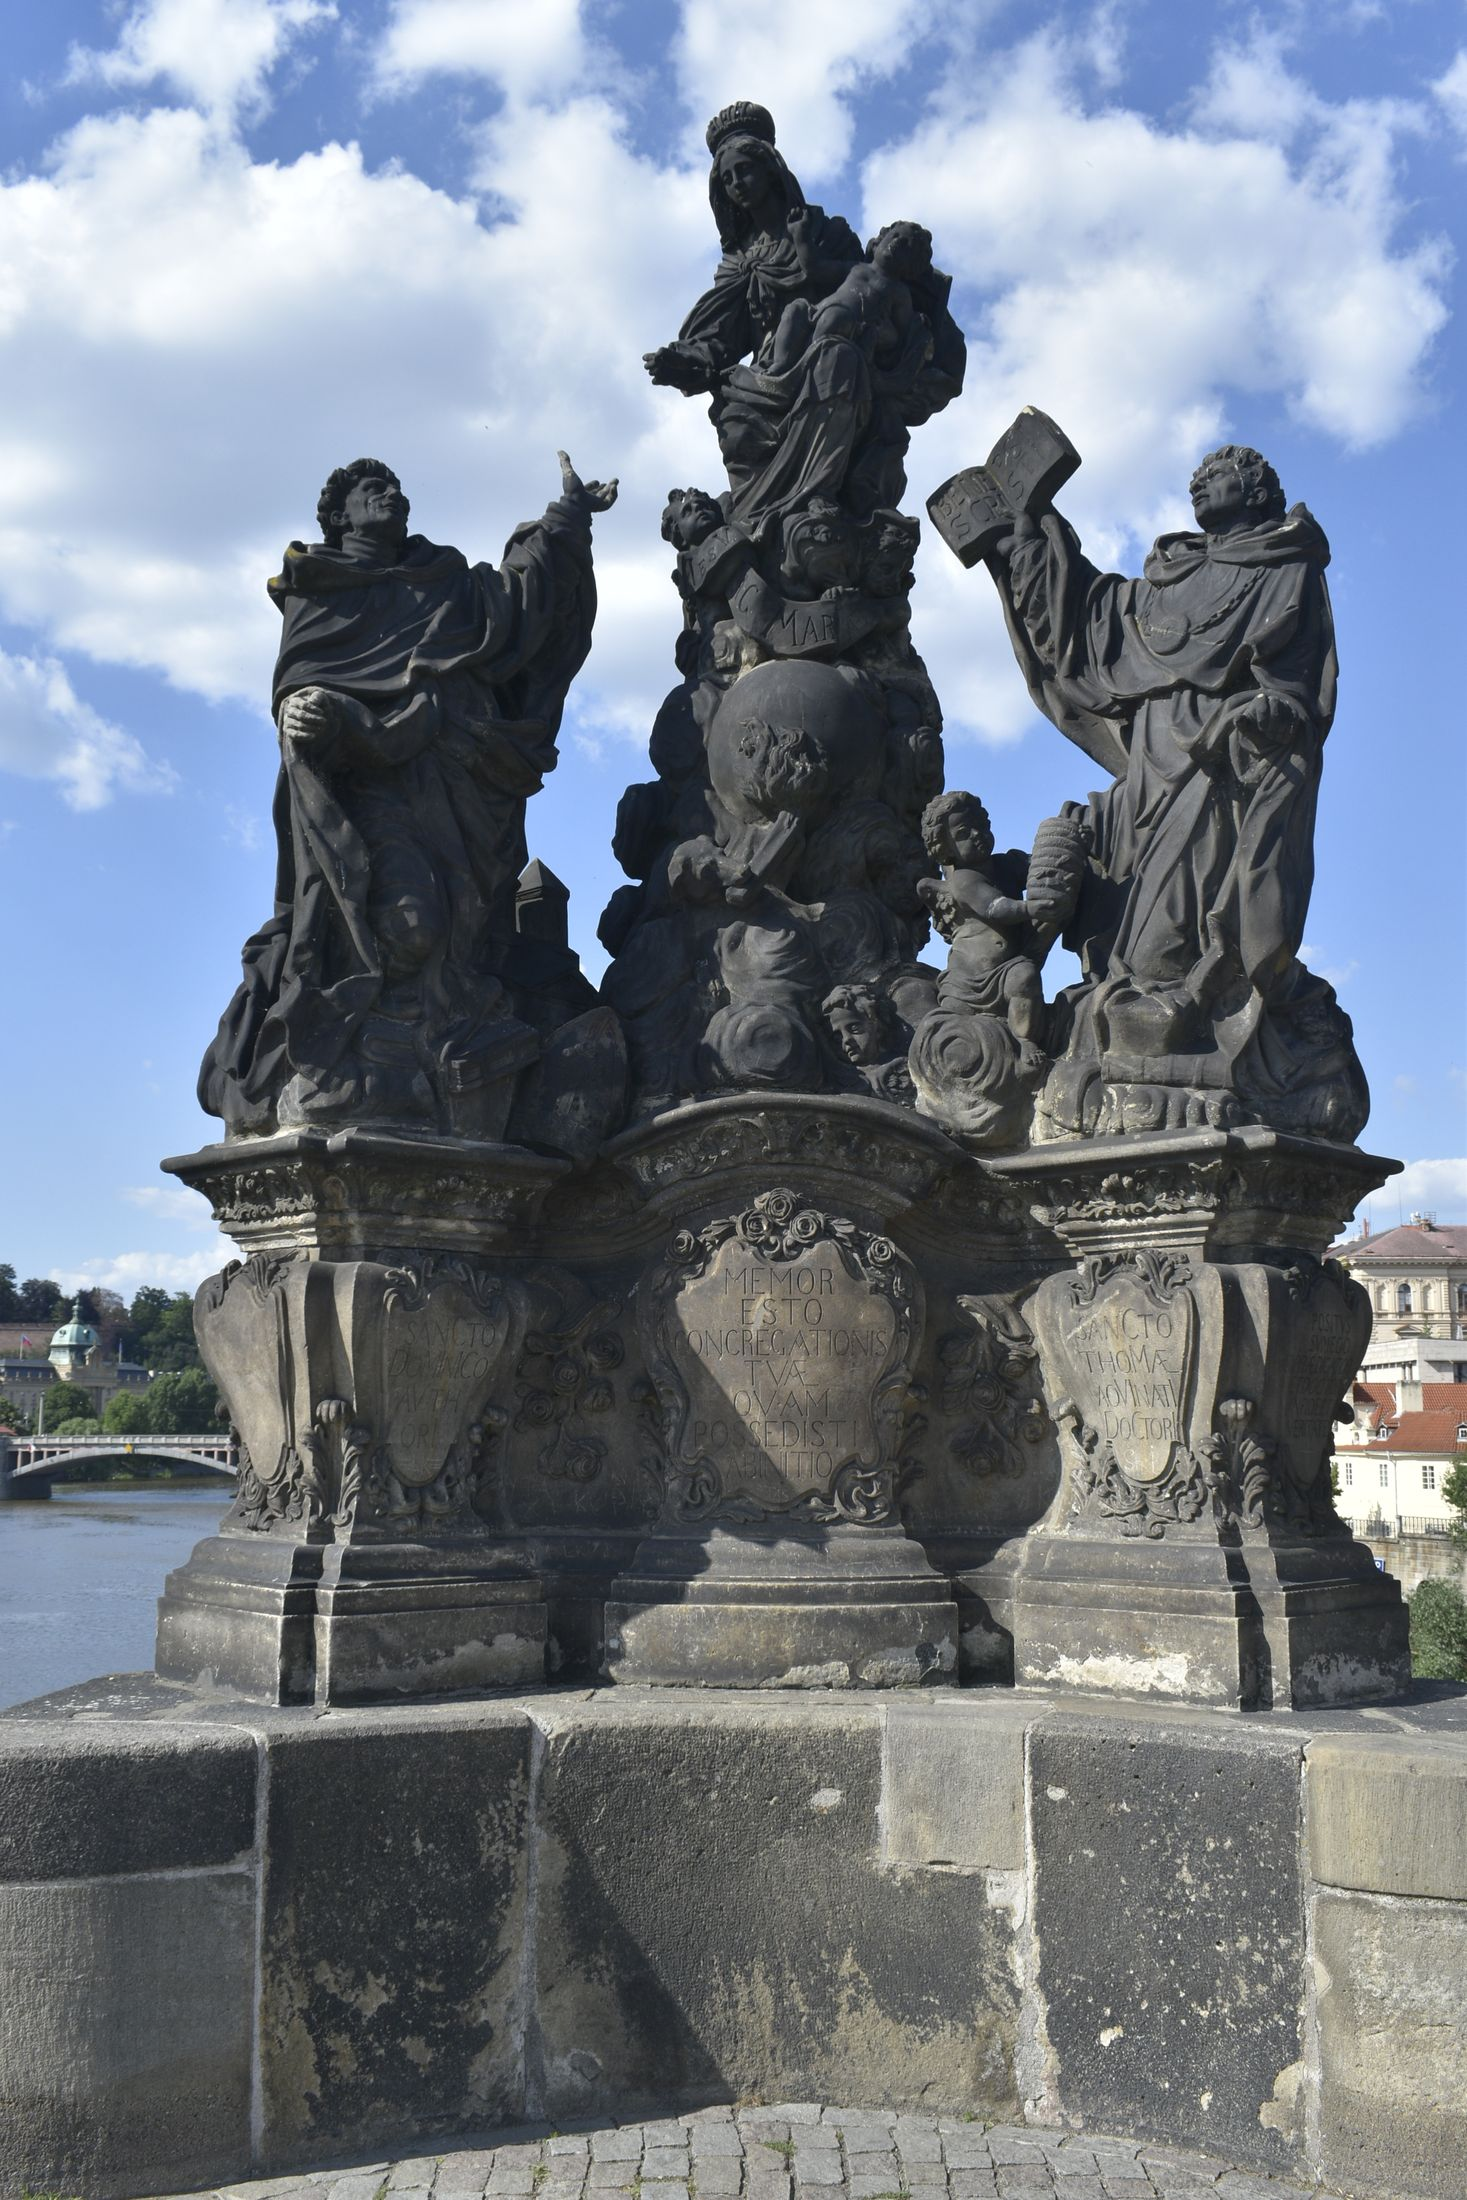
\includegraphics[height=2.10in,width=1.55in,viewport=5 3 1550 2180,clip]{Figures/Madonna-Ss.-Dominic-and-Thomas_Aquinas-3.jpeg}
\hspace*{15pt}
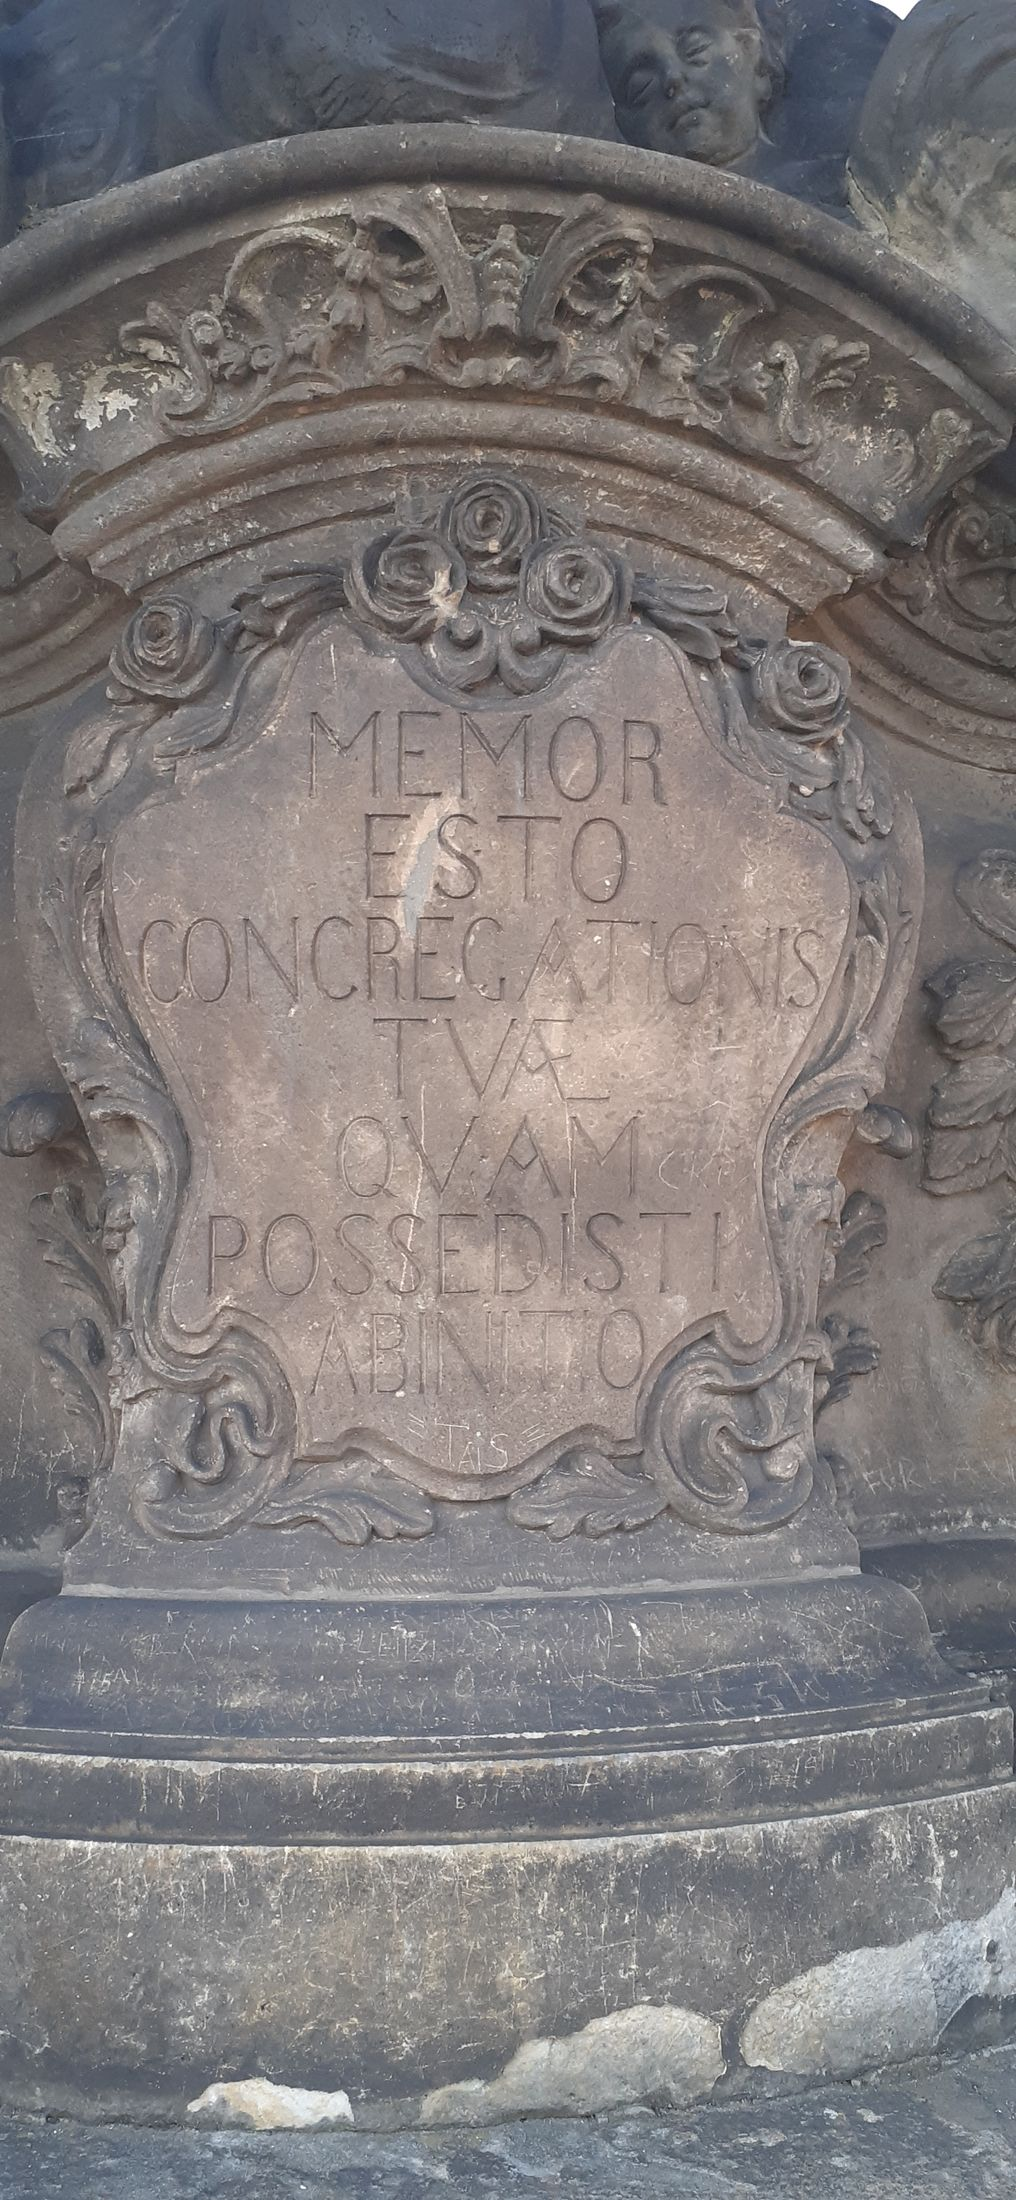
\includegraphics[height=2.10in,width=1.15in,viewport=5 3 950 1880,clip]{Figures/Madonna-Ss.-Dominic-and-Thomas_Aquinas-Inscription_2.jpeg}
%\caption{\tiny \textrm{Pseudopotential for metallic sodium, based on the empty core model and screened by the Thomas-Fermi dielectric function.}}%(与文献\cite{EPJB33-47_2003}图1对比)
\label{ABINITIO-inscription}
\end{figure}
\begin{minipage}{0.53\textwidth}
	{\fontsize{8.2pt}{4.2pt}\selectfont{ 
		\centering{MEMOR}\\
		\centering{ESTO}\\
		\centering{CONGREGATIONIS}\\
		\centering{TV\AE}\\
		\centering{QVAM}\\
		\centering{POSSEDISTI}\\
		\centering{\textcolor{red}{ABINITIO}\\}}}
\end{minipage}
\hspace*{5pt}
\begin{minipage}{0.30\textwidth}
	\textrm{\fontsize{4.2pt}{4.2pt}\selectfont{The inscription in English:}}\\
	\textrm{\fontsize{8.2pt}{4.2pt}\selectfont{\textcolor{blue}{Mind the congregation that has been yours} \textcolor{purple}{since the beginning}}}
\end{minipage}
}

\frame
{
	\frametitle{电荷密度代替电子}
\begin{figure}[h!]
\centering
\vspace{3.5pt}
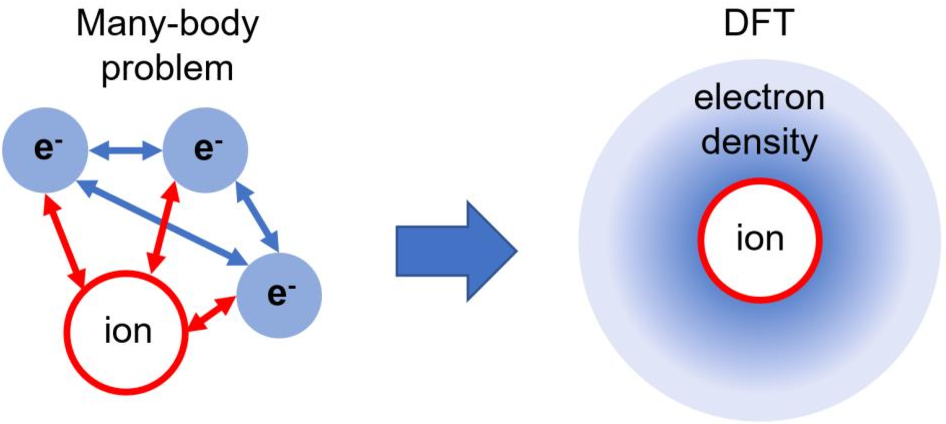
\includegraphics[height=0.45\textwidth,width=1.0\textwidth,viewport=0 0 950 440,clip]{Figures/Schematic-illustration-of-transforming-many_electron-system-to-electron-density.png}
\caption{\fontsize{6.0pt}{4.5pt}\selectfont{\textrm{Schematic illustration of transforming many-electron system to electron density.}}}
\label{Density-Particle}
\end{figure}
}

%\section{密度泛函理论}       %Bookmark
\frame
{
	\frametitle{\rm{Creators of DFT}}
\begin{figure}[h!]
\vskip 10pt
\centering
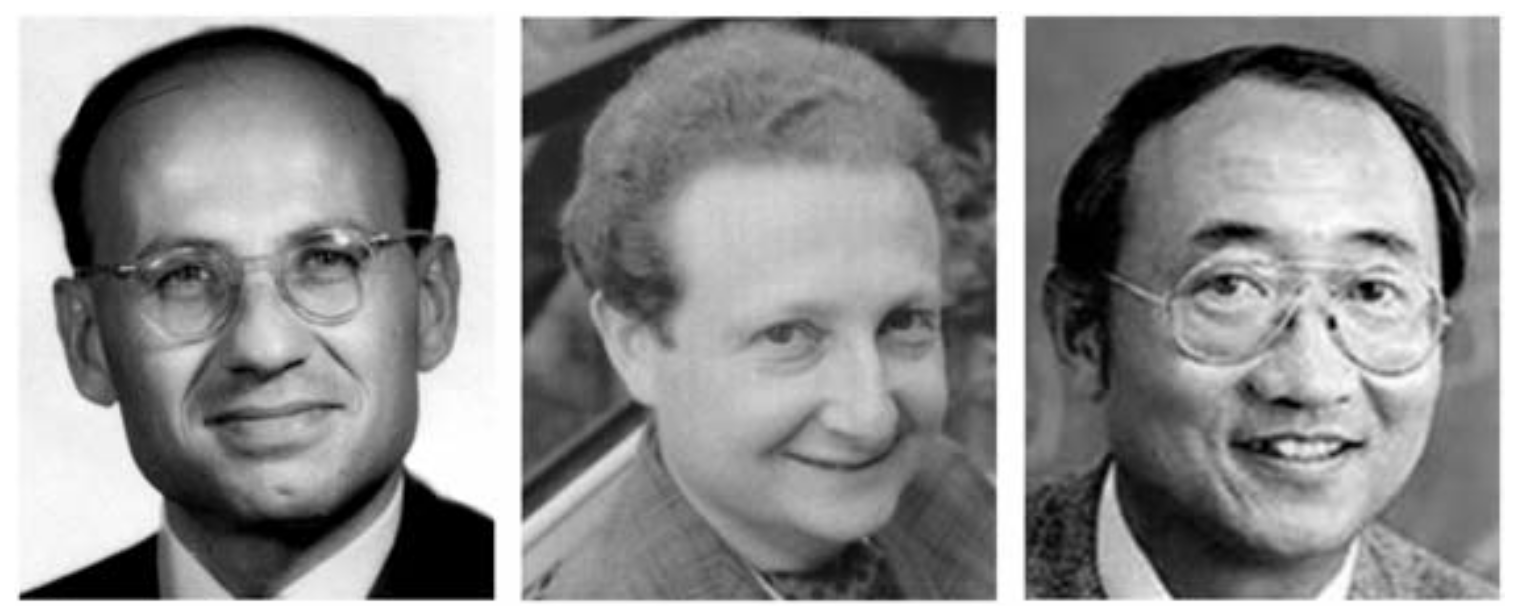
\includegraphics[height=1.65in,width=4.0in,viewport=0 0 1562 610,clip]{Figures/Creators_of_DFT.png}
\caption{\tiny \textrm{Creators of DFT. Walter Kohn(left, in 1962) and his two postdoctoral fellows, Pierre Hohenberg (middle, in 1965) and Lujeu Sham (right).}}%(与文献\cite{EPJB33-47_2003}图1对比)
\label{Creator_of_DFT}
\end{figure}
}

\frame                               %
{
	\frametitle{\textrm{Kohn-Sham}方程}
\begin{figure}[h!]
\centering
\vspace*{-0.21in}
\hspace*{-0.1in}
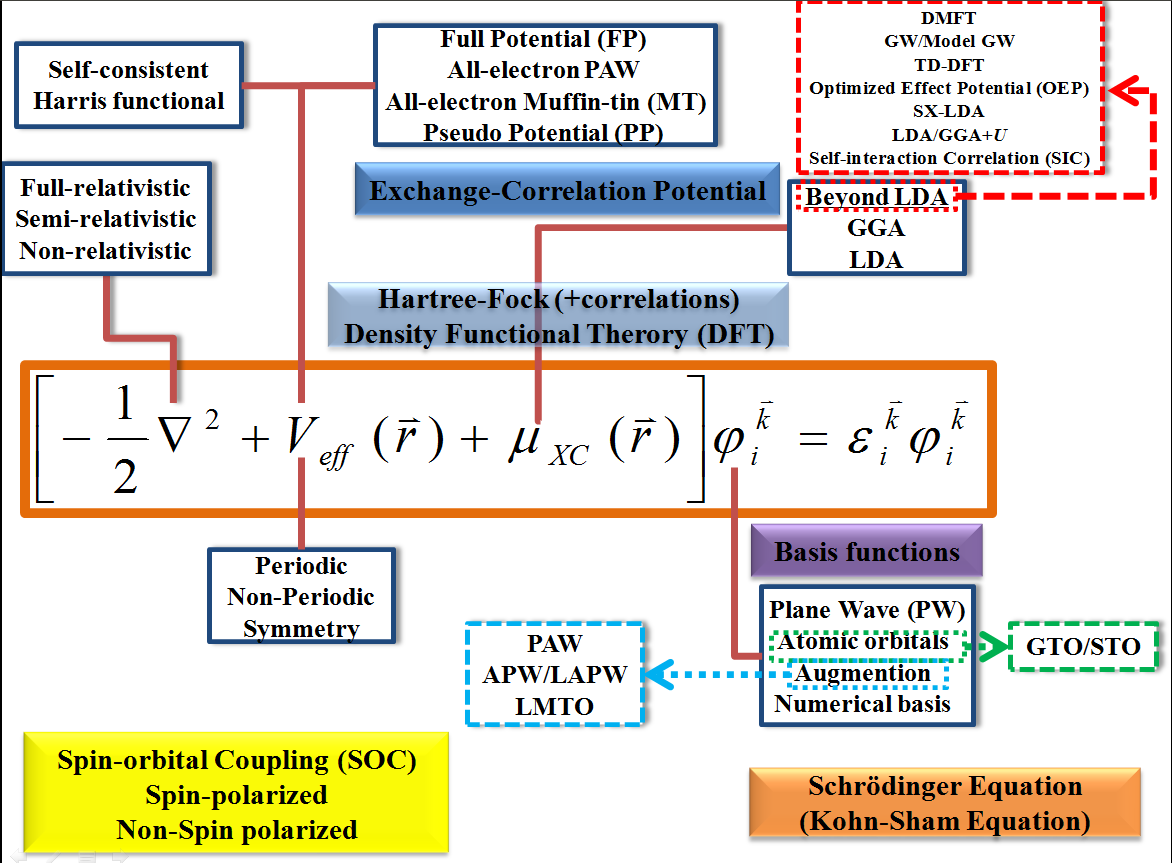
\includegraphics[height=2.7in,width=4.0in,viewport=2 5 1162 880,clip]{Figures/DFT.png}
\caption{\tiny \textrm{The Analysis of Kohn-Sham equation.}}%(与文献\cite{EPJB33-47_2003}图1对比)
\label{DFT}
\end{figure}
}

\frame
{
	\frametitle{密度\textrm{vs.}粒子与泛函表示}
\begin{figure}[h!]
\vskip -10pt
\centering
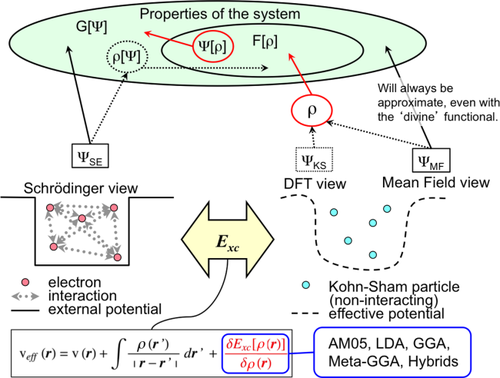
\includegraphics[height=2.65in,width=3.8in,viewport=0 0 362 275,clip]{Figures/DFT-particle-density.png}
\caption{\fontsize{6.0pt}{4.5pt}\selectfont{\textrm{Properties of a quantum mechanical system can be calculated by solving the SE (left). A more tractable, formally equivalent way is to solve the DFT KS equations (right).}}}%(与文献\cite{EPJB33-47_2003}图1对比)
\label{Schrodinger-equation-vs-Kohn-Sham-equation}
\end{figure}
}

\frame                               %
{
	\frametitle{近似能量泛函$E_{\mathrm{XC}}[\rho]$的主要问题}
\vskip 20pt
\begin{enumerate}%[+-| alert@+>]
   \setlength{\itemsep}{10pt}
 \item  密度是整体变量:~电子自相互作用抵消不净\\%\quad\textrm{(LDA+U)}方法的校正%(\textrm{LDA+U})
	 用\textrm{DFT}计算电子数很少的体系,一般都会有较大的误差
 \item  电子相关:~简并和近简并基态的表示不合理\\
	 基态电子密度用不同的简并轨道计算时,体系能量应保持不变,但现有的近似能量泛函不具有这个性质
 \item  渐近行为:~处理弱相互作用体系的误差大\\
	 如\textrm{Van der Waals}相互作用和现有近似能量泛函本身的计算误差在同一量级
 \end{enumerate}
}

\subsection{从理论到软件的实现}
\frame
{
	\frametitle{\textrm{DFT-SCF}}
\begin{figure}[h!]
\centering
\vspace*{-0.25in}
\hspace*{-0.80in}
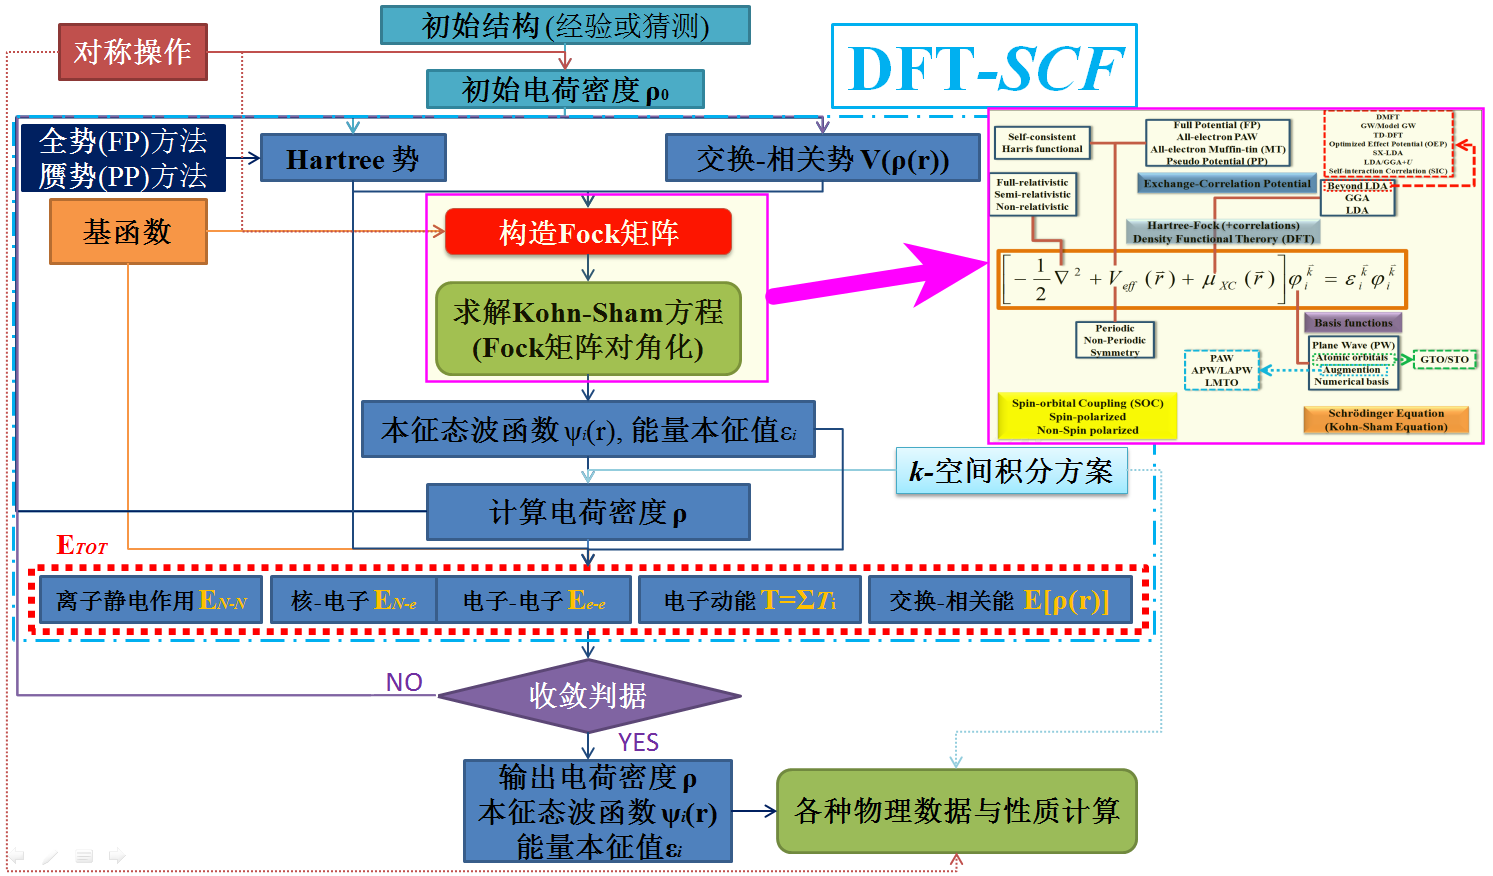
\includegraphics[height=2.80in,width=4.95in,viewport=5 3 1490 870,clip]{Figures/DFT-SCF_2.png}
%\caption{\tiny \textrm{Pseudopotential for metallic sodium, based on the empty core model and screened by the Thomas-Fermi dielectric function.}}%(与文献\cite{EPJB33-47_2003}图1对比)
\label{DFT-SCF-2}
\end{figure}
}

\frame
{
	\frametitle{晶体总能量的一般表示}
采用赝势方法计算的晶体总能量$E_T$由晶格中的电子能量$E_{e-e}$与离子实排斥能$E_{N-N}$之和:
	\begin{displaymath}
		E_T=E_{e-e}+E_{N-N}=T[\rho]+E_{ext}+E_{\mathrm{Coul}}+E_{\mathrm{XC}}+E_{N-N}
	\end{displaymath}
根据\textrm{Kohn-Sham}方程,其中动能泛函用单电子能量表示为
\begin{displaymath}
	T[{\rho}]=\sum_in_i\langle\psi_i|\varepsilon_i-V_{\mathrm{KS}}|\psi_i\rangle
\end{displaymath}
$n_i$是$\psi_i$上的电子占据数,$\varepsilon_i$是其能量本征值,因此有
\begin{displaymath}
	\hspace*{-12.0pt}	E_T=\sum_in_i\varepsilon_i-\dfrac12\int\int\mathrm{d}\vec r\mathrm{d}\vec r\dfrac{\rho(\vec r)\rho(\vec r^{\prime})}{|\vec r-\vec r^{\prime}|}+\int\mathrm{d}\vec r\rho(\vec r)[\epsilon_{\mathrm{XC}}(\vec r)-V_{\mathrm{XC}}(\vec r)]+E_{N-N}
\end{displaymath}
}

\frame
{
	\frametitle{晶体总能量倒空间的表示}
周期体系的总能量表达式在动量空间($\vec K$空间)计算更方便
\begin{displaymath}
	\hspace*{-15.0pt}	E_T=\textcolor{red}{\sum_in_i\varepsilon_i}-\dfrac{\Omega}2\sum_{\textcolor{red}{\vec k\neq 0}}\rho^{\ast}(\vec k)V_{\mathrm{Coul}}(\vec k)+\Omega\sum_{\vec k}\rho^{\ast}(\vec k)[\epsilon_{\mathrm{XC}}(\vec k)-V_{\mathrm{XC}}(\vec k)]+E_{N-N}
\end{displaymath}
其中$V_{\mathrm{Coul}}(\vec k)$、$\epsilon_{\mathrm{XC}}(\vec k)$与$\rho^{\ast}(\vec k)$分别是\textrm{Coulomb}相互作用、单个电子的交换-相关能、交换-相关势和电子密度的\textrm{Fourier}分量。

由\textrm{Poisson}方程
\begin{displaymath}
	\nabla^2V_{\mathrm{Coul}}(\vec r)=-4\pi\rho(\vec r)
\end{displaymath}
的\textrm{Fourier}展开有
\begin{displaymath}
	V_{\mathrm{Coul}}(\vec k)=\dfrac{4\pi\rho^{\ast}(\vec k)}{|\vec k|^2}
\end{displaymath}
交换-相关势和交换-相关能的计算一般先在实空间计算$\epsilon_{\mathrm{XC}}(\vec r)$和$V_{\mathrm{XC}}(\vec r)$后,再通过\textrm{Fourier}变换到动量空间,得到$\epsilon_{\mathrm{XC}}(\vec k)$和$V_{\mathrm{XC}}(\vec k)$
}

\subsection{$\vec k$~空间布点与积分}
\frame
{
	\frametitle{$\vec k$~空间布点与\textrm{Fermi~}面的确定}
\begin{figure}[h!]
\centering
\hspace*{-0.35in}
\subfigure[\textrm{Brillouin Zone of Cubic lattice}]{
\label{Brillouin_Zone_Cubic-2}
\vspace*{-0.50in}
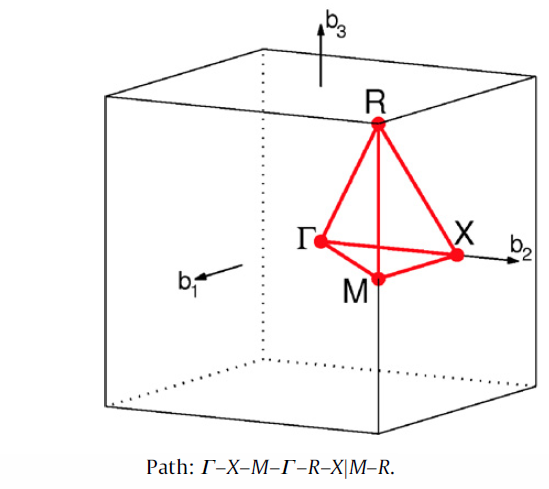
\includegraphics[height=2.10in,width=2.00in,viewport=90 0 550 500,clip]{Figures/Brillouin-Zone_CUB.png}}
\subfigure[\textrm{Band Structure of SrSnO$_3$}]{
\label{Band_Gap_SrSnO3-2}
\vspace*{-0.50in}
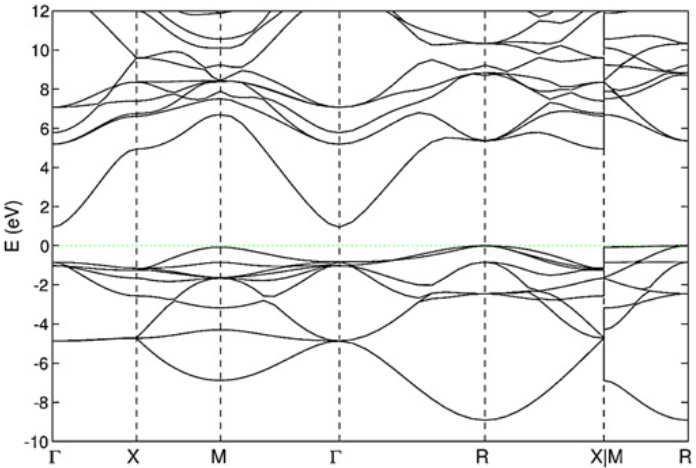
\includegraphics[height=2.10in,width=1.95in,viewport=0 0 710 550,clip]{Figures/Band-Struct_SrSnO3.png}}
\label{Band_Gap_CUB_SrSnO3}
\end{figure}
在固体能带理论中,\textcolor{blue}{能量色散关系$\varepsilon(\vec k)$}~表示能量在倒空间中分布,其中量子数$\vec k$~(晶体动量)描述平移对称性
%\textcolor{blue}{能带图表示能量在\textrm{Brillouin-zone~}特定方向的色散关系}
}

\frame
{
	\frametitle{$\vec k$~空间布点与\textrm{Fermi~}面的确定}
\begin{figure}[h!]
\centering
%\hspace*{-10pt}
\vspace*{-0.3in}
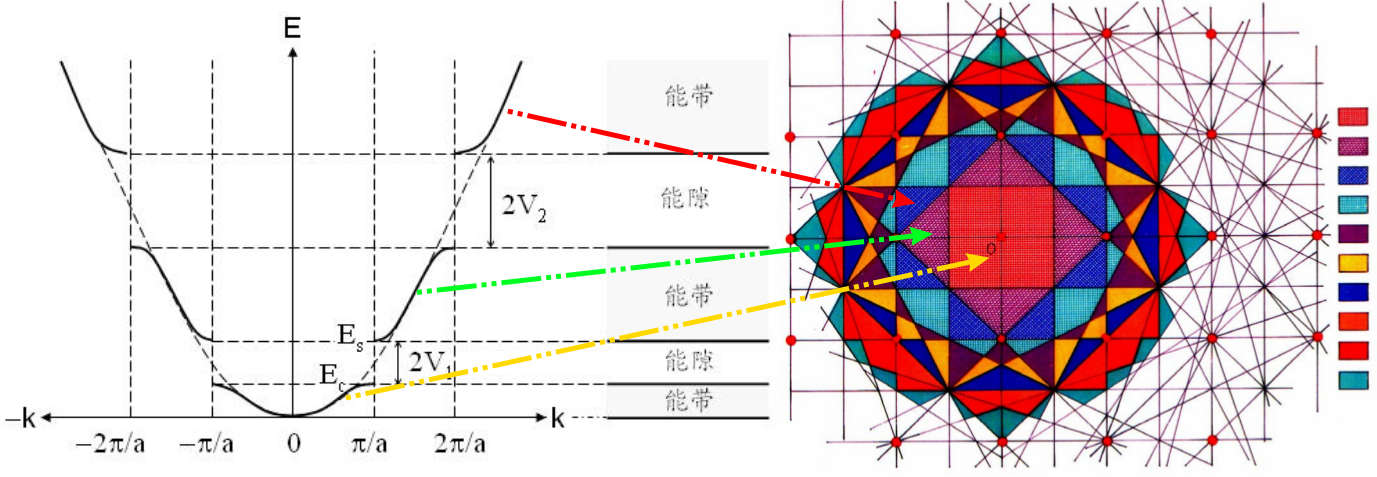
\includegraphics[height=1.5in,width=4.1in,viewport=0 5 1400 500,clip]{Figures/Brillouin-Band.png}
\caption{\tiny \textrm{The relation between unfolded-Band and the Brillouin-zone.}}%
\label{Brillouin-Band}
\end{figure} 
周期体系的\textrm{Fermi~}能级和\textrm{Fermi~}面的确定:\\
\begin{displaymath}
	\left\{
	\begin{aligned}
		&\mbox{\textcolor{red}{导体:~}}&\mbox{\textcolor{blue}{价电子在\textrm{Brillouin-zone~}部分填充}}\\
		&\mbox{\textcolor{red}{半导体-绝缘体:~}}&\mbox{\textcolor{blue}{价电子在\textrm{Brillouin-zone~}完全填充}}
	\end{aligned}\right.
\end{displaymath}
}

\frame
{
	\frametitle{$\vec k$~空间布点与\textrm{Fermi~}面的确定}
\begin{figure}[h!]
\centering
%\hspace*{-10pt}
\vspace*{-0.15in}
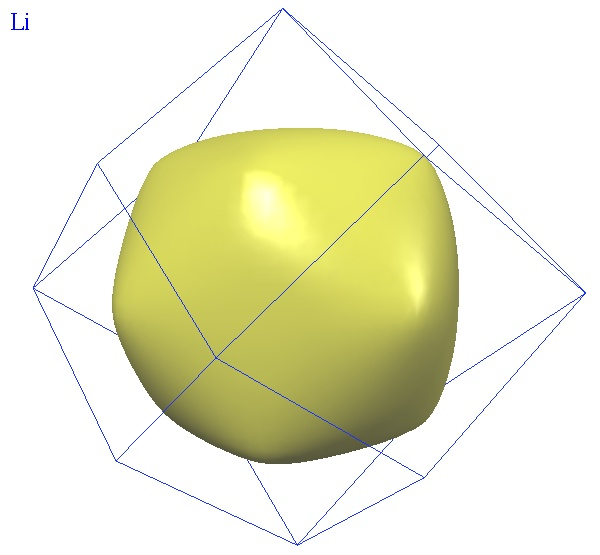
\includegraphics[height=1.2in,width=1.3in,viewport=0 0 110 100,clip]{Figures/FS-Li.jpg}
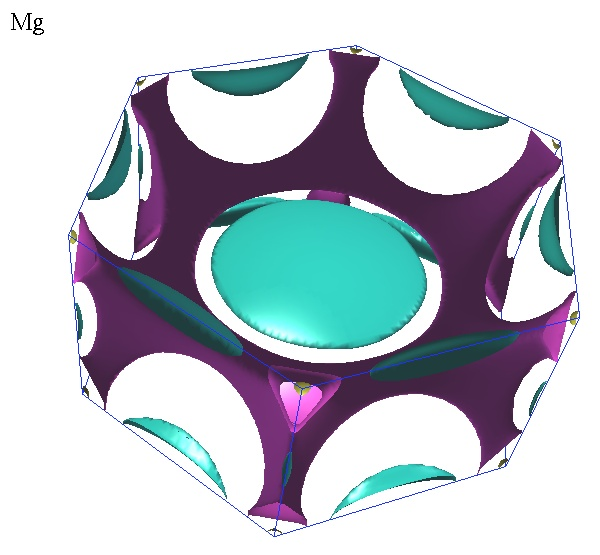
\includegraphics[height=1.2in,width=1.3in,viewport=0 0 110 100,clip]{Figures/FS-Mg.jpg}
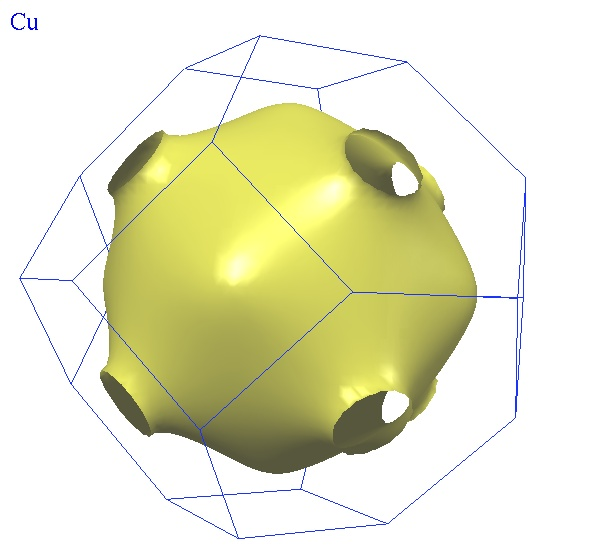
\includegraphics[height=1.2in,width=1.3in,viewport=0 0 110 100,clip]{Figures/FS-Cu.jpg}
\caption{\tiny \textrm{The Fermi-surface of Li, Mg, Cu in the first Brillouin-zone.}}%
\label{Brillouin-Band-Fermi}
\end{figure} 
\textcolor{blue}{\textrm{Fermi~}面的形状}:\\
\textcolor{red}{最高占据能带折叠到第一\textrm{Brillouin-zone~}围成的区域}

\vspace{10pt}
要确定\textrm{Fermi~}面的精细结构,\underline{\textcolor{red}{特别是对于金属和导体体系}},必须在整个\textrm{Brillouin-zone~}取足够多的采样点
}

\frame
{
\frametitle{$\vec k$~空间积分与物理量计算}
与\textrm{Fermi~}面的确定类似,周期体系中所有单粒子期望值可表示为整个\textrm{Brillouin-zone~}内占据态的矩阵元的积分\\

一般地,如果已知\textrm{Brillouin-zone~}某点$\vec k$~的能带指标为$n$的波函数本征态$\Psi_n(\vec k)$~和本征值$\epsilon_n(\vec k)$,算符$\mathbf{X}$~的期望值$\langle X \rangle$是矩阵元
\begin{displaymath}
	X_n(\vec k)=\langle\Psi_n(\vec k)|\mathbf{X}|\Psi_n(\vec k)\rangle 
\end{displaymath}
\textcolor{blue}{在倒空间全部占据能带的求和}
\begin{displaymath}
	\langle X\rangle=\dfrac1{\sqrt V_G}\sum_n\int_{V_G}\mathrm{d}^3kX_n(\vec k)f(\varepsilon_n(\vec k))
\end{displaymath}
其中$V_G$是第一\textrm{Brillouin-zone}体积,$f(\varepsilon)$~是占据分布函数

实际计算中,\textrm{Brillouin-zone~}的$\vec k$~点数是有限的
\begin{displaymath}
	\langle X\rangle=\sum_{j,n}X_n(\vec k_j)w_n^{\vec k_j}
\end{displaymath} 
\textcolor{blue}{$\vec k$~点数目决定了电子结构和物理量的的精度与计算量}
}

\frame
{
\frametitle{$\vec k$~空间布点方案}
\begin{enumerate}
	\item \textcolor{red}{简单分布函数}\\
		\begin{itemize}
			\item 
				\begin{figure}[h!]
					\begin{minipage}[t]{0.40\linewidth}
						\textrm{Fermi-Dirac~}分布函数$$f(\varepsilon)=\dfrac1{\mathrm{e}^{(\varepsilon-\mu)/kT}+1}$$ 
						其中$\mu$是化学势,$k$~是\textrm{Boltzmann}常数,$T$是温度参数
					\end{minipage}
				\hfill
					\begin{minipage}[t]{0.55\linewidth}
					\centering
					\vspace*{-0.35in}
					\hspace*{-0.5in}
					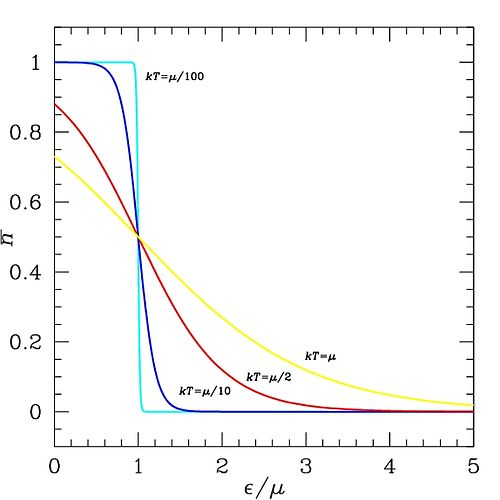
\includegraphics[height=1.0in,width=1.25in,viewport=0 0 530 500,clip]{Figures/Fermi-Dirac-distribution.jpg}
					\caption{\textrm{The Fermi-Dirac Distribution.}}%
					\label{Fermi-Dirac-distribution}
					\end{minipage}
					%\hspace*{-10pt}
				\end{figure} 
			\item 
				\begin{figure}[h!]
					\begin{minipage}[t]{0.40\linewidth}
						\textrm{Gaussian~}分布函数$$f(\varepsilon)=\dfrac1{\sigma\sqrt{2\pi}}\mathrm{e}^{-\frac{(\varepsilon-\mu)^2}{2\sigma^2}}$$
						其中$\mu$是化学势,$\sigma$是展宽参数
					\end{minipage}
				\hfill
					\begin{minipage}[t]{0.55\linewidth}
					\centering
					\vspace*{-0.35in}
					\hspace*{-0.5in}
					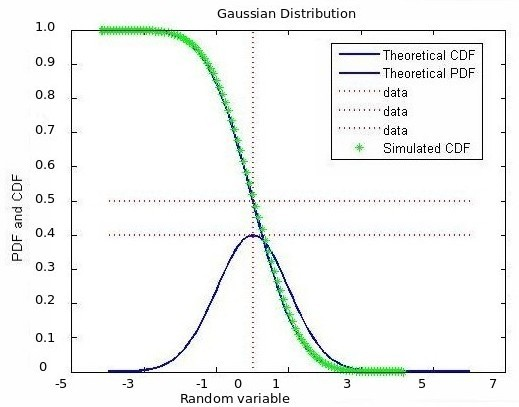
\includegraphics[height=1.0in,width=1.25in,viewport=0 0 530 500,clip]{Figures/Gaussian-distribution.jpg}
					\caption{\tiny \textrm{The Gaussian Distribution.}}%
					\label{Gaussian-distribution}
					\end{minipage}
					%\hspace*{-10pt}
				\end{figure} 
%			\item \textrm{Lorentz~}分布函数$$L(x)=\frac1{\pi}\frac{\frac12\Gamma}{(x-x_0)^2+\left(\frac12\Gamma\right)^2}$$
%				这里$x_0$是中心,$\Gamma$是展宽参数
		\end{itemize}
\end{enumerate}
}

\frame
{
\frametitle{$\vec k$~空间布点方案}
\begin{enumerate}
	\setcounter{enumi}{1}
	\item \textcolor{red}{特殊点方法\textrm{(Special-point scheme)}}\\这是一种相对高效的积分方法,通过选取少量有代表性的$\vec k$~点,即可获得较高的计算精度,这些$\vec k$~点被称为“平均值点”或“特殊点”\\特殊点方法对导体的收敛性较差
\begin{figure}[h!]
\centering
%\hspace*{-10pt}
%\vspace*{-0.2in}
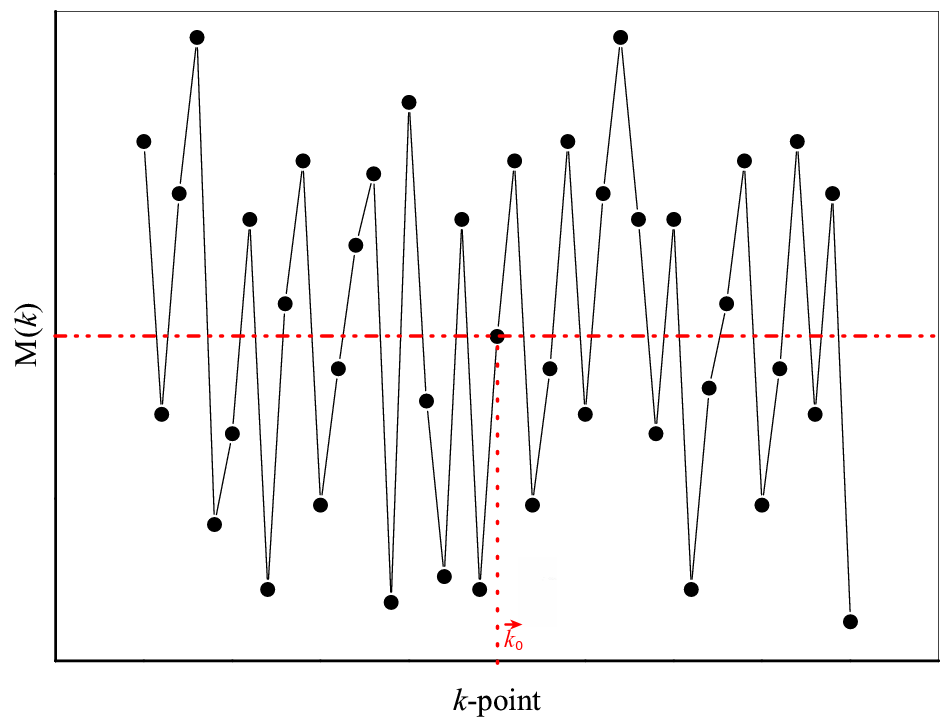
\includegraphics[height=1.6in,width=1.8in,viewport=5 0 960 750,clip]{Figures/Brillouin-k.png}
\caption{\tiny \textrm{The mean value and the $\vec k$-point.}}%
\label{Brillouin-k}
\end{figure} 
\end{enumerate}
}

\frame
{
	\frametitle{\textrm{Monkhorst-Pack}布点方案}
	\begin{itemize}
		\item 最初的特殊点方案必须首先确定$2\sim3$个性能较好的$\vec k$~点,由此构建$\vec k$~点集合拥有比较高的效率和精度,所以每个具体体系,计算前必须经过相当的对称性分析。从程序编写角度来说,非常麻烦
		\item \textrm{Monkhorst-Pack}提出一套简易的$\vec k$~点网格生成方法:

\begin{figure}[h!]
\begin{minipage}[t]{0.55\linewidth}
			\textrm{Monkhorst-Pack}简易按如下方案划分\textrm{Brillouin-zone}:
			$$\boxed{u_r=\dfrac{(2r-q-1)}{2q}\quad(r=1,2,3,\cdots,q)}$$
			$q$是确定特殊点数目的某个整数
			\vspace{-0.1in}
			$$A_m(\vec k)=N_m^{-1/2}\sum_{|\vec R|=C_m}\mathrm{e}^{\mathrm{i}\vec k\cdot\vec R}$$
\end{minipage}
\hfill
\begin{minipage}[t]{0.42\linewidth}
\centering
%\hspace*{2pt}
\vspace*{-0.6in}
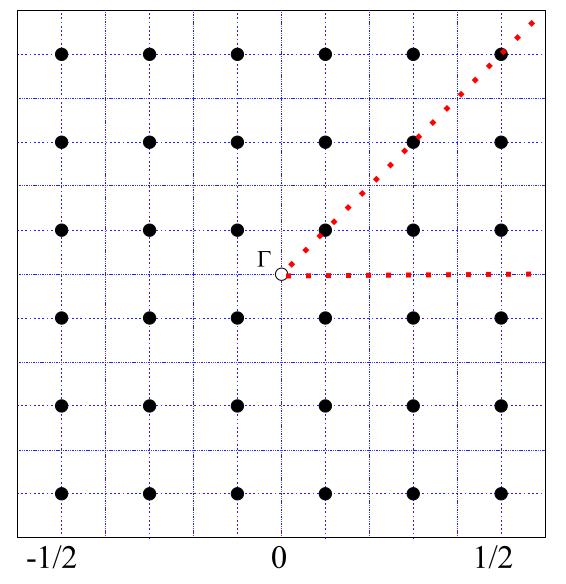
\includegraphics[height=1.5in,width=2.05in,viewport=-200 0 850 800,clip]{Figures/Special-points-MP.png}
\caption{\tiny \textrm{The generation of special $\vec k$-points in \textrm{Monkhorst-Pack} method.}}%
\label{Special-points-MP}
\end{minipage}
\end{figure} 
	\end{itemize}
}

\frame
{
\frametitle{$\vec k$~空间布点方案}
\begin{enumerate}
	\setcounter{enumi}{2}
	\item \textcolor{red}{四面体方法\textrm{(Tetrahedron schemen)}}\\这是一种线性插值方法,将\textrm{Brillouin-zone~}用体积相等的四面体填充,在每个四面体内部,被积函数$X_n(\vec k_j)$和能量$\varepsilon_n^{\vec k_j}$都随$\vec k$~点线性变化\\一般来说,四面体方法对金属和导体的\textrm{Fermi~}面确定更可靠
\begin{figure}[h!]
\centering
%\vspace*{-0.25in}
	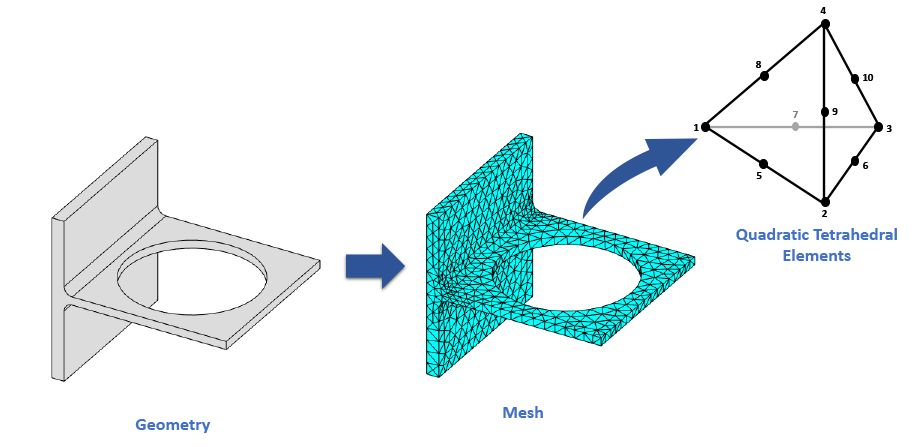
\includegraphics[height=1.55in,width=3.15in,viewport=30 0 900 500,clip]{Figures/Finite_element_analysis.jpg}
	\caption{\tiny \textrm{Schematic representation of a finite element method FEM-model.}}%(与文献\cite{EPJB33-47_2003}图1对比)
\label{Fig:FEM}
\end{figure}
\end{enumerate}
}


\frame
{
	\frametitle{各种$\vec k$~空间积分方法的比较}
\vskip -7pt
\begin{footnotesize}
\arrayrulewidth=0.4pt
\doublerulesep=0.4pt
\begin{table}[!h]
\tabcolsep 0pt \vspace*{-12pt}
%\begin{minipage}{\textwidth}
\label{tab:magno-1}
\centering
\def\temptablewidth{1.01\textwidth}
{\rule{\temptablewidth}{0.8pt}}
\begin{tabular*} {\temptablewidth}{|c@{\extracolsep{\fill}}|c|c|c|c|}
	\multirow{3}{*}{\textcolor{red}{积分方案}}	&\multicolumn{4}{c|}{\textcolor{blue}{布点方案}:~\textrm{Monkhorst-Pack}~方法} \\\cline{2-5}
	&\multirow{2}{*}{\textrm{Fermi-Dirac}~方法} &\multicolumn{2}{c|}{\textrm{Methfessel-Paxton}~方法} &\multirow{2}{*}{\textrm{Tetrahedron}~方法}\\\cline{3-4}
& &\textrm{Gaussian~} &$N>0$ & \\ \hline
半导体、&\multirow{2}{*}{\textcolor{blue}{$\texttimes$}} &$\delta\leqslant0.05$ &\multirow{2}{*}{\textcolor{red}{$\texttimes$}} &\textcolor{blue}{\textrm{DOS \& total-Energy}}\\
绝缘体 & &\textcolor{blue}{$\checkmark$} & &\textcolor{red}{$\checkmark$} \\\hline
导体、 & \multirow{2}{*}{\textcolor{blue}{$\checkmark$}} & \multicolumn{2}{c|}{\textcolor{blue}{\textrm{Phonon \& relaxation}}} &\textcolor{blue}{\textrm{DOS \& total-Energy}} \\
金属 & &\multicolumn{2}{c|}{\textcolor{red}{$\checkmark$}}  &\textcolor{red}{$\checkmark$} \\\hline
\multirow{2}{*}{\textrm{supercell}} &\multirow{2}{*}{\textcolor{blue}{$\checkmark$}} &\multicolumn{2}{c|}{\multirow{2}{*}{\textcolor{red}{$\checkmark$}}} &\multirow{2}{*}{\textcolor{red}{$\texttimes$}}\\
& &\multicolumn{2}{c|}{} &\\
\end{tabular*}
{\rule{\temptablewidth}{1pt}}\\
%\end{center}1
%\end{minipage}
\end{table}
\end{footnotesize}
\textcolor{purple}{如何方便地确定每个$\vec k$~点的积分权重$w_n^{\vec k_i}$,精确、高效地完成\textrm{Brillouin-zone~}积分是$\vec k$~空间布点方案的主要研究内容}
}
%\frame
%{
%\begin{figure}[h!]
%\centering
%\vspace*{-0.25in}
%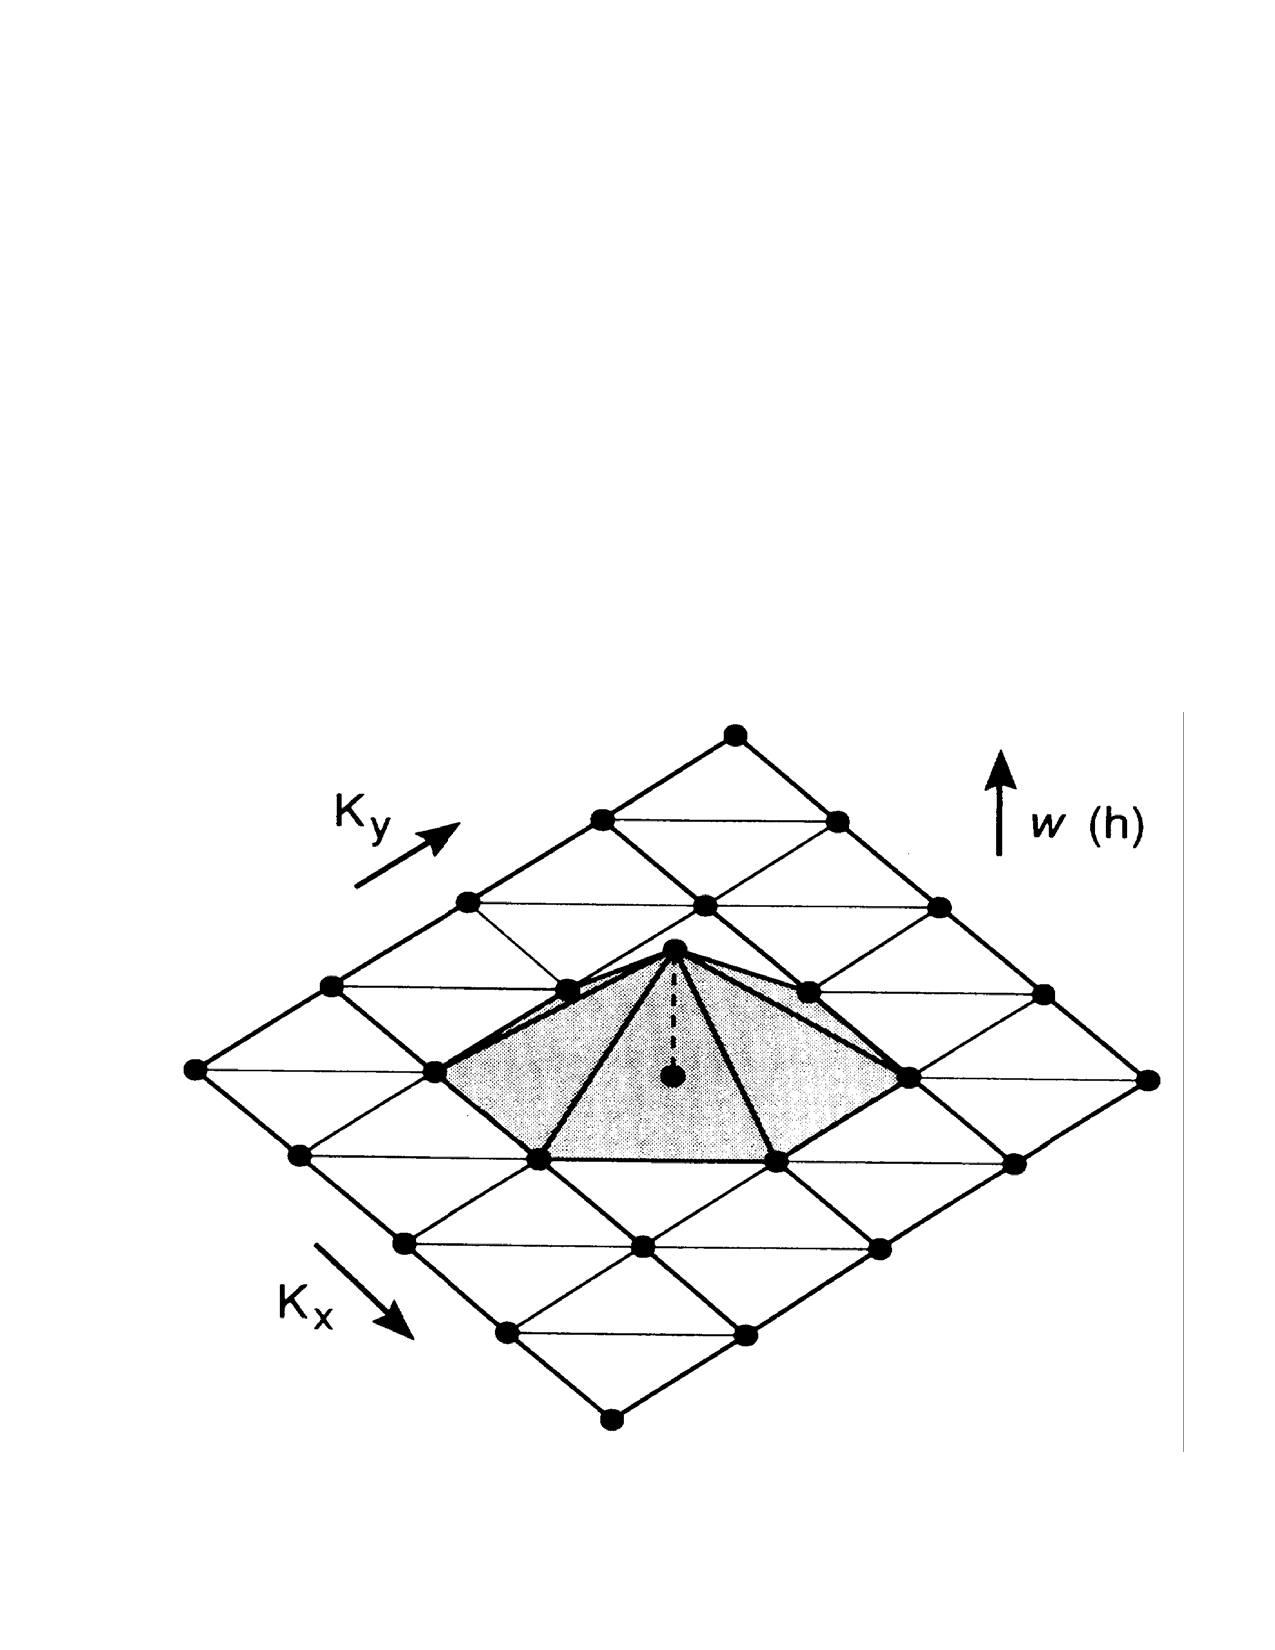
\includegraphics[height=2.75in,width=3.05in,viewport=0 30 565 505,clip]{Figures/dimen_Tetra.pdf}
%\caption{\tiny Two-dimensional schematic illustration of the function $w_j(\vec k)$.}%(与文献\cite{EPJB33-47_2003}图1对比)
%\label{Fig:dime_Tetra-2}
%\end{figure}
%}

\subsection{计算方法与软件分类}       %Bookmark
\frame
{
	\frametitle{基组:~张开空间,展开波函数}
\begin{figure}[h!]
	\vspace{-5pt}
\centering
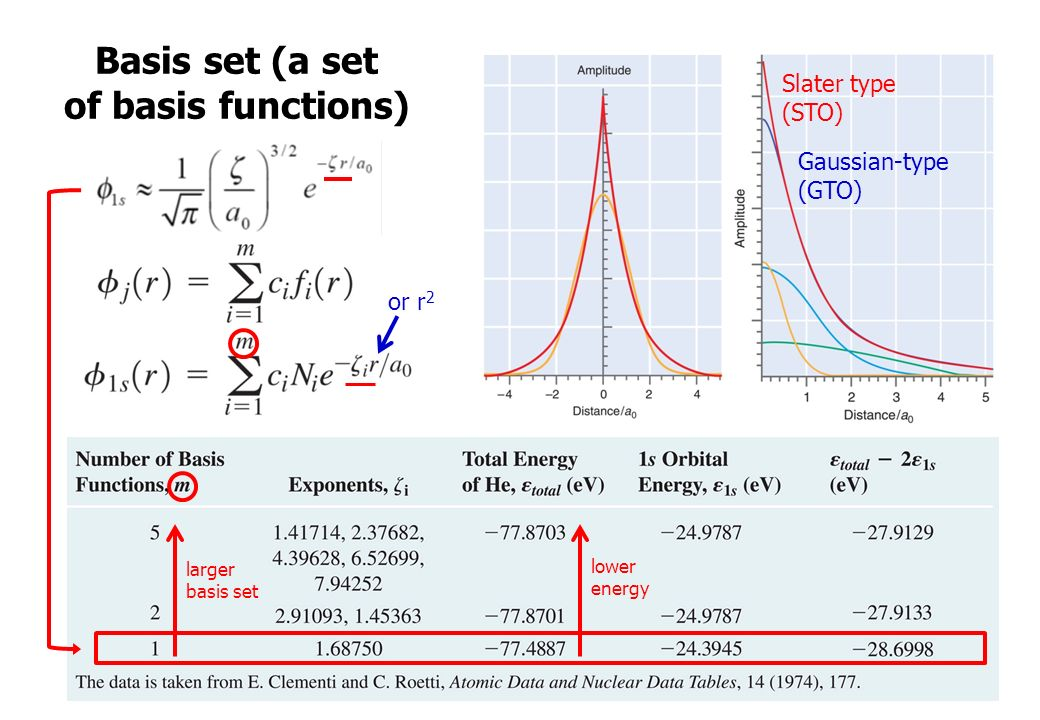
\includegraphics[height=2.6in,width=4.01in,viewport=0 0 780 550,clip]{Figures/Basis-set-STO-GTO.jpg}
\caption{\fontsize{5.5pt}{4.2pt}\selectfont{\textrm{Schematic illustration of scattering of a Basic-set STO GTO.}}}%(与文献\cite{EPJB33-47_2003}图1对比)
\label{Basic-set:STO-GTO}
\end{figure}
}

\frame
{
%\frametitle{The methods on band structure calculation}
\frametitle{固体能带计算方法}
%\vskip 10pt
%\textrm{The mainly difference of all these methods below: the basis sets and the construction of the potential}
\vskip 10pt
常用的固体能带计算方法
\begin{itemize}%[+-| alert@+>]
%\begin{enumerate}%[+-| alert@+>]
\setlength{\itemsep}{12pt}
%  \item \textrm{Plane wave and the pseudo-potential}
	\item	平面波方法
	\item	正交平面波\textrm{(The orthogonalized plane wave, OPW)}和赝势\textrm{(Pseudo-potential, PP)}方法\upcite{Singh,PRB41-7892_1990,JPCM6-8245_1994}
	\item	缀加平面波\textrm{(Augmented plane wave, APW)}方法
	\item	\textrm{MT}轨道\textrm{(Muffin-tin orbitals, MTO)}方法\upcite{LMTO_Book}
	\item	投影子缀加波\textrm{(Projector Augmented Wave, PAW)}方法\upcite{PRB50-17953_1994,PRB59-1758_1999}
\end{itemize}
\vskip 5pt 各种方法的\textcolor{red}{主要区别}:~\textcolor{blue}{势函数的处理}与\textcolor{blue}{所选基函数类型}不同
}

\frame
{
	\frametitle{固体计算软件概览}
\begin{figure}[h!]
\centering
\vspace*{-0.05in}
%\hspace*{-0.80in}
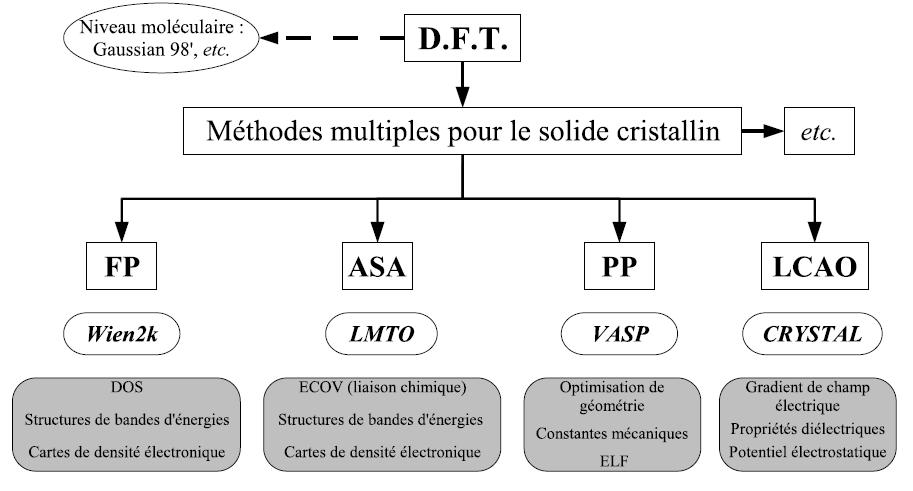
\includegraphics[height=2.30in,width=4.00in,viewport=0 0 920 500,clip]{Figures/DFT-Software.jpg}
%\caption{\tiny \textrm{Pseudopotential for metallic sodium, based on the empty core model and screened by the Thomas-Fermi dielectric function.}}%(与文献\cite{EPJB33-47_2003}图1对比)
\label{Abinitio-Softwares}
\end{figure}
}

\section{软件解方程:~迭代与优化}
\frame
{
	\frametitle{非线性方程的\rm{Newton~}法求根}
	\textcolor{blue}{不管哪一种数值算法,其设计原理都是将复杂转化为简单的重复,或者说,通过简单的重复生成复杂}:\\
	\textcolor{red}{在算法设计和算法实现过程中,重复就是力量}\\
迭代算法设计:~\textcolor{purple}{“速度”\textrm{vs}“稳定”}
\begin{figure}[h!]
\centering
\animategraphics[autoplay, loop, height=2.0in]{1}{Figures/OP_Newton_}{0}{17}
\label{Equation_Newon}
\end{figure}
}

\frame
{
	\frametitle{迭代优化基本思想}
	对于给定函数$f$,在极值点,函数的梯度满足
	\begin{displaymath}
		\nabla f=0
	\end{displaymath}
	可将函数极值问题转化成方程求根问题
\begin{figure}[h!]
\centering
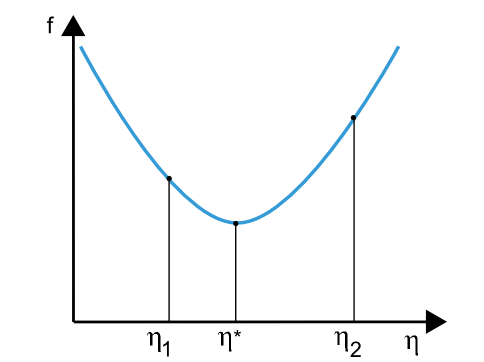
\includegraphics[height=1.68in,width=1.95in,viewport=30 0 450 360,clip]{Figures/OP_mini-1.png}
\hskip 0.05in
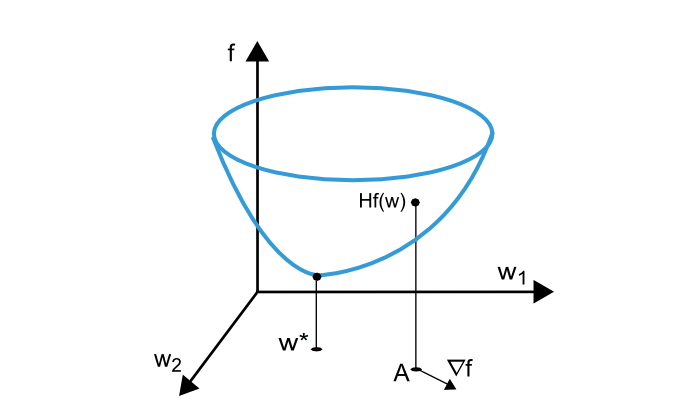
\includegraphics[height=1.68in,width=1.95in,viewport=150 20 560 390,clip]{Figures/OP_mini-2.png}
\label{OP_mini}
\end{figure}
}

\frame
{
	\frametitle{最陡下降与共轭梯度}
\begin{figure}[h!]
\centering
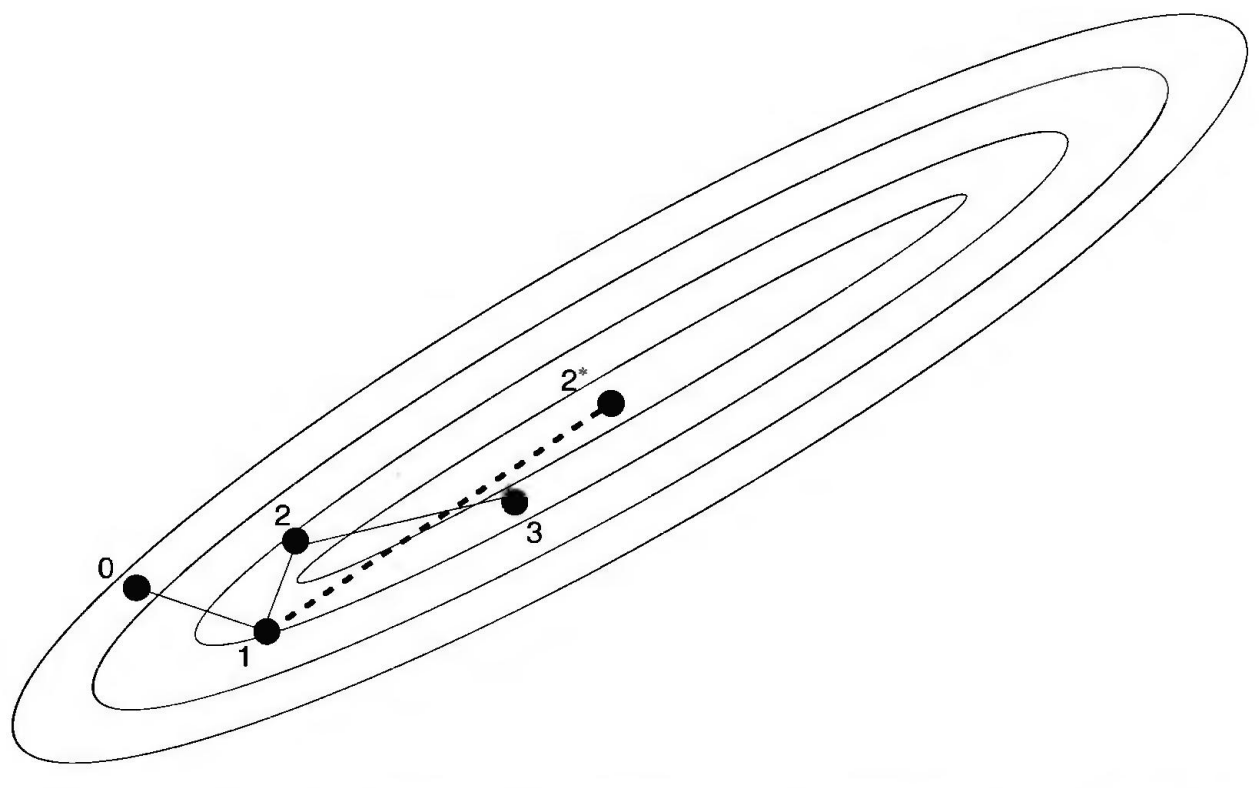
\includegraphics[height=2.0in,width=3.5in,viewport=0 0 950 590,clip]{Figures/OP_descent_CG.png}
\label{decent_CG}
\caption{\tiny \textrm{Schematic illustration of minimization of a function in two dimensions. The steps 1,2,3,~$\cdots$ denote the steepest descent steps and the point - \!- \!- \!- \!- \!- denote the conjugate gradient path that reaches the exact solution after two steps if the functional is quadratic.}}%(与文献\cite{EPJB33-47_2003}图1对比)
\end{figure}
}

\frame
{
	\frametitle{共轭梯度的``轭''}
\begin{figure}[h!]
\centering
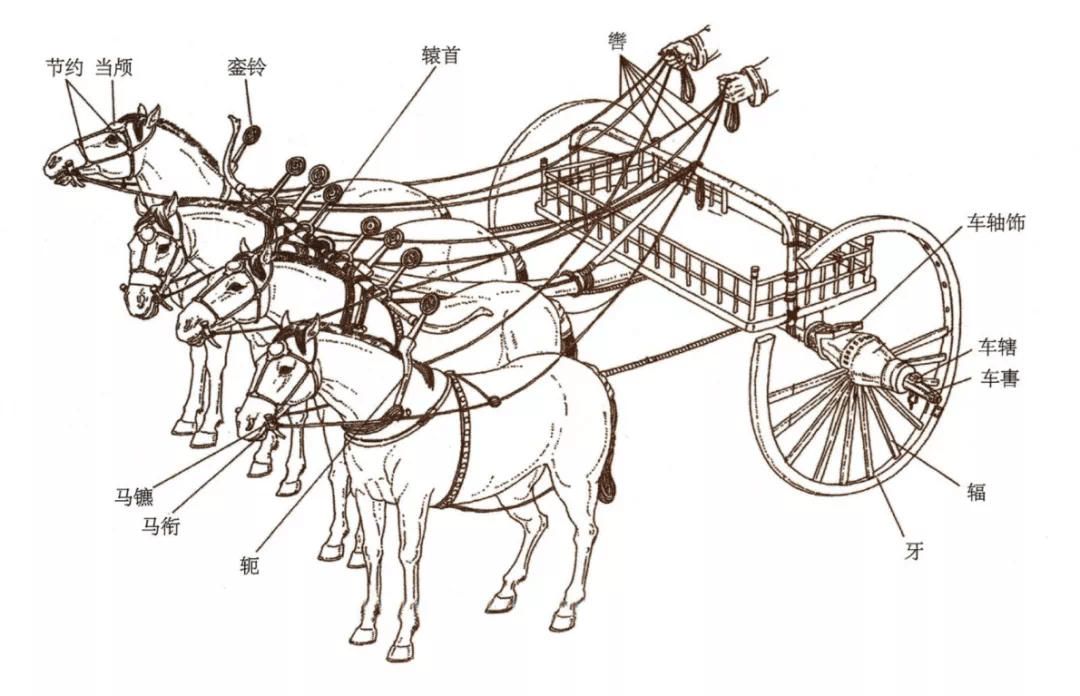
\includegraphics[height=2.5in,width=4.0in,viewport=0 0 1050 680,clip]{Figures/Yoke_1.png}
\label{Horse_Yoke}
%\caption{\tiny \textrm{Schematic illustration of minimization of a function in two dimensions. The steps 1,2,3,$\cdots$ denote the steepest descent steps and the point $2^{\ast}$ denote the conjugate gradient path that reaches the exact solution after two steps if the functional is quadratic.}}%(与文献\cite{EPJB33-47_2003}图1对比)
\end{figure}
}

\frame
{
	\frametitle{共轭的含义}
\begin{minipage}{0.63\textwidth}
\begin{figure}[h!]
\vskip -23pt
\centering
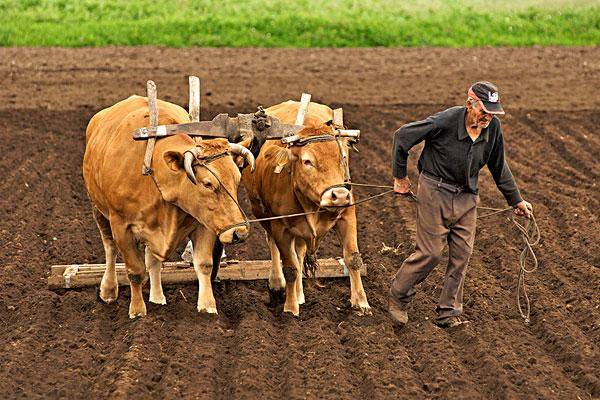
\includegraphics[height=1.6in,width=2.2in,viewport=0 0 600 490,clip]{Figures/Bi-Yoke_1.jpg}
\vskip 2pt
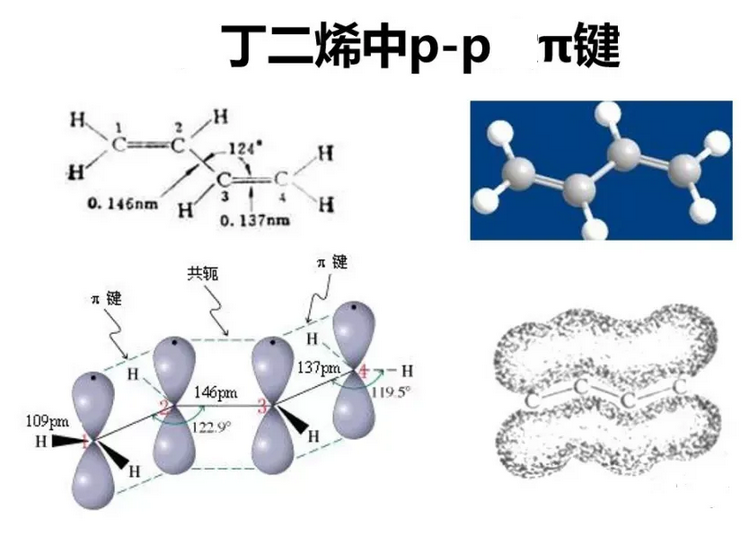
\includegraphics[height=1.5in,width=2.2in,viewport=0 0 750 530,clip]{Figures/Conjugate_Pi-bond.png}
\label{Conjugate_1}
%\caption{\tiny \textrm{Schematic illustration of minimization of a function in two dimensions. The steps 1,2,3,$\cdots$ denote the steepest descent steps and the point $2^{\ast}$ denote the conjugate gradient path that reaches the exact solution after two steps if the functional is quadratic.}}%(与文献\cite{EPJB33-47_2003}图1对比)
\end{figure}
\end{minipage}
\begin{minipage}{0.35\textwidth}
\begin{figure}[h!]
\centering
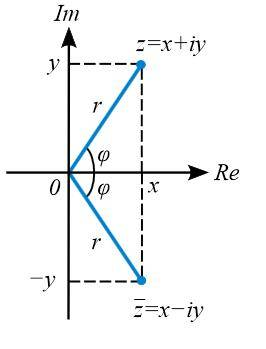
\includegraphics[height=2.2in,width=1.5in,viewport=0 0 250 390,clip]{Figures/Conjugate_complex.jpg}
\label{Conjugate_2}
%\caption{\tiny \textrm{Schematic illustration of minimization of a function in two dimensions. The steps 1,2,3,$\cdots$ denote the steepest descent steps and the point $2^{\ast}$ denote the conjugate gradient path that reaches the exact solution after two steps if the functional is quadratic.}}%(与文献\cite{EPJB33-47_2003}图1对比)
\end{figure}
\end{minipage}
}

		\frame[allowframebreaks]
{
\frametitle{主要参考文献}
\begin{thebibliography}{99}
{\tiny
        \bibitem{Singh}\textrm{D. J. Singh. \textit{Plane Wave, PseudoPotential and the LAPW method} (Kluwer Academic, Boston,USA, 1994)}					%
	\bibitem{PRB41-7892_1990}\textrm{D. Vanderbilt. \textit{Phys. Rev.} B, \textbf{41} (1990), 7892} 
	\bibitem{JPCM6-8245_1994}\textrm{G. Kresse and J. Hafner. J. Phys: \textit{Condens. Matter}, \textbf{6} (1994), 8245}
	\bibitem{LMTO_Book}\textrm{H. Skriver. \textit{The LMTO method} (Springer, New York, USA, 1984)}
	\bibitem{PRB50-17953_1994}\textrm{P. E. Bl\"ochl. \textit{Phys. Rev.} B, \textbf{50} (1994), 17953}
	\bibitem{PRB59-1758_1999}\textrm{G. Kresse and D. Joubert \textit{Phys. Rev.} B, \textbf{59} (1999), 1758}
	\bibitem{Andersen_Book}\textrm{O. K. Andersen. \textit{Computational Methods in Band Theory} (Plenum, New York, USA, 1971)}
	\bibitem{Nemoshkalenko-Antonov}\textrm{V. V. Nemoshkalenko and V. N. Antonov. \textit{Computational Methods in Solid State Physics} (Gordon and Breach Science Publisher, Amsterdam, The Netherlands, 1998)}
	\bibitem{Xie-Lu}谢希德、陆栋\:主编, {\textit{固体能带理论}}\:复旦大学出版社, 上海, 1998
	\bibitem{Elect_Stru}\textrm{Richard. M. Martin. \textit{Electronic Structure: Basic Theory and Practical Methods} (Cambridge University Press, Cambridge, England, 2004)}
	\bibitem{Comp_Phys}\textrm{J. M. Thijssen. \textit{Computational Physics}~\textrm{(2nd Edition)} (Cambridge University Press, Cambridge, England, 2007)}
}
\end{thebibliography}
}

\section{计算示例:~\rm{VASP}}
\frame
{
	\frametitle{\textrm{VASP}软件简介}
	\textrm{VASP}软件是维也纳大学\textrm{(Universit\"at Wien)}~\textrm{G. Kresse}等开发的第一原理模拟软件包
	\begin{itemize}
		\item \textrm{VASP}采用\textrm{PAW~(Projector Augmented-Wave)}方法,平衡了赝势方法和全电子计算优点,兼顾了计算的精度和效率
		\item \textrm{VASP}在实空间优化投影函数\textrm{(Projector)},将主要的计算过程变换到实空间完成,大大节省了内存的开销%,保证了计算精度和效率
		\item \textrm{VASP}通过引入多样的优化算法,提高了矩阵对角化和电荷密度搜索的效率
		\item 在\textrm{VASP}的并行计算中,有效均衡了各节点处理\textrm{FFT}变换负载和通信,提升了软件的并行效率
	\end{itemize}
	相比于其他第一原理计算软件,\textrm{VASP}从物理思想与方法、优化算法和并行计算实现等多个方面都有更为出色的性能
}

\frame
{
	\frametitle{\textrm{VASP}的开发团队}
\begin{figure}[h!]
\centering
\vspace*{-0.25in}
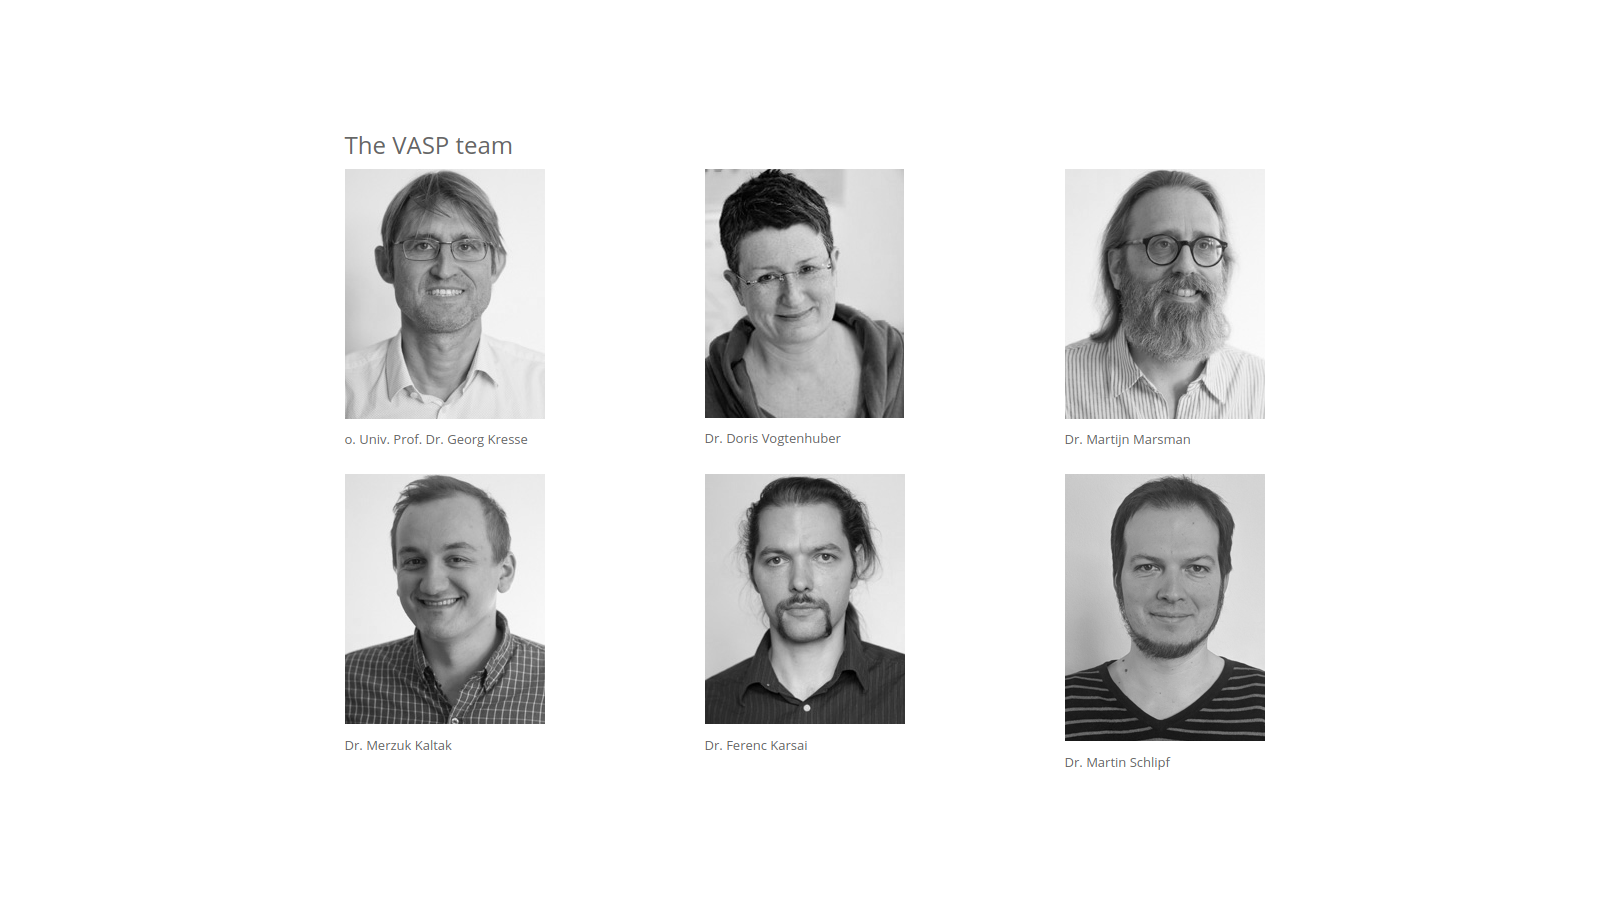
\includegraphics[height=2.70in,width=4.05in,viewport=330 130 1280 770,clip]{Figures/VASP_team.png}
\caption{\tiny \textrm{The development team of VASP.}}%(与文献\cite{EPJB33-47_2003}图1对比)
\label{VASP_team}
\end{figure}
}

\frame
{
	\frametitle{\textrm{VASP}的\textrm{Kohn-Sham}方程求解流程}
\begin{figure}[h!]
	\vspace{-0.2in}
\centering
%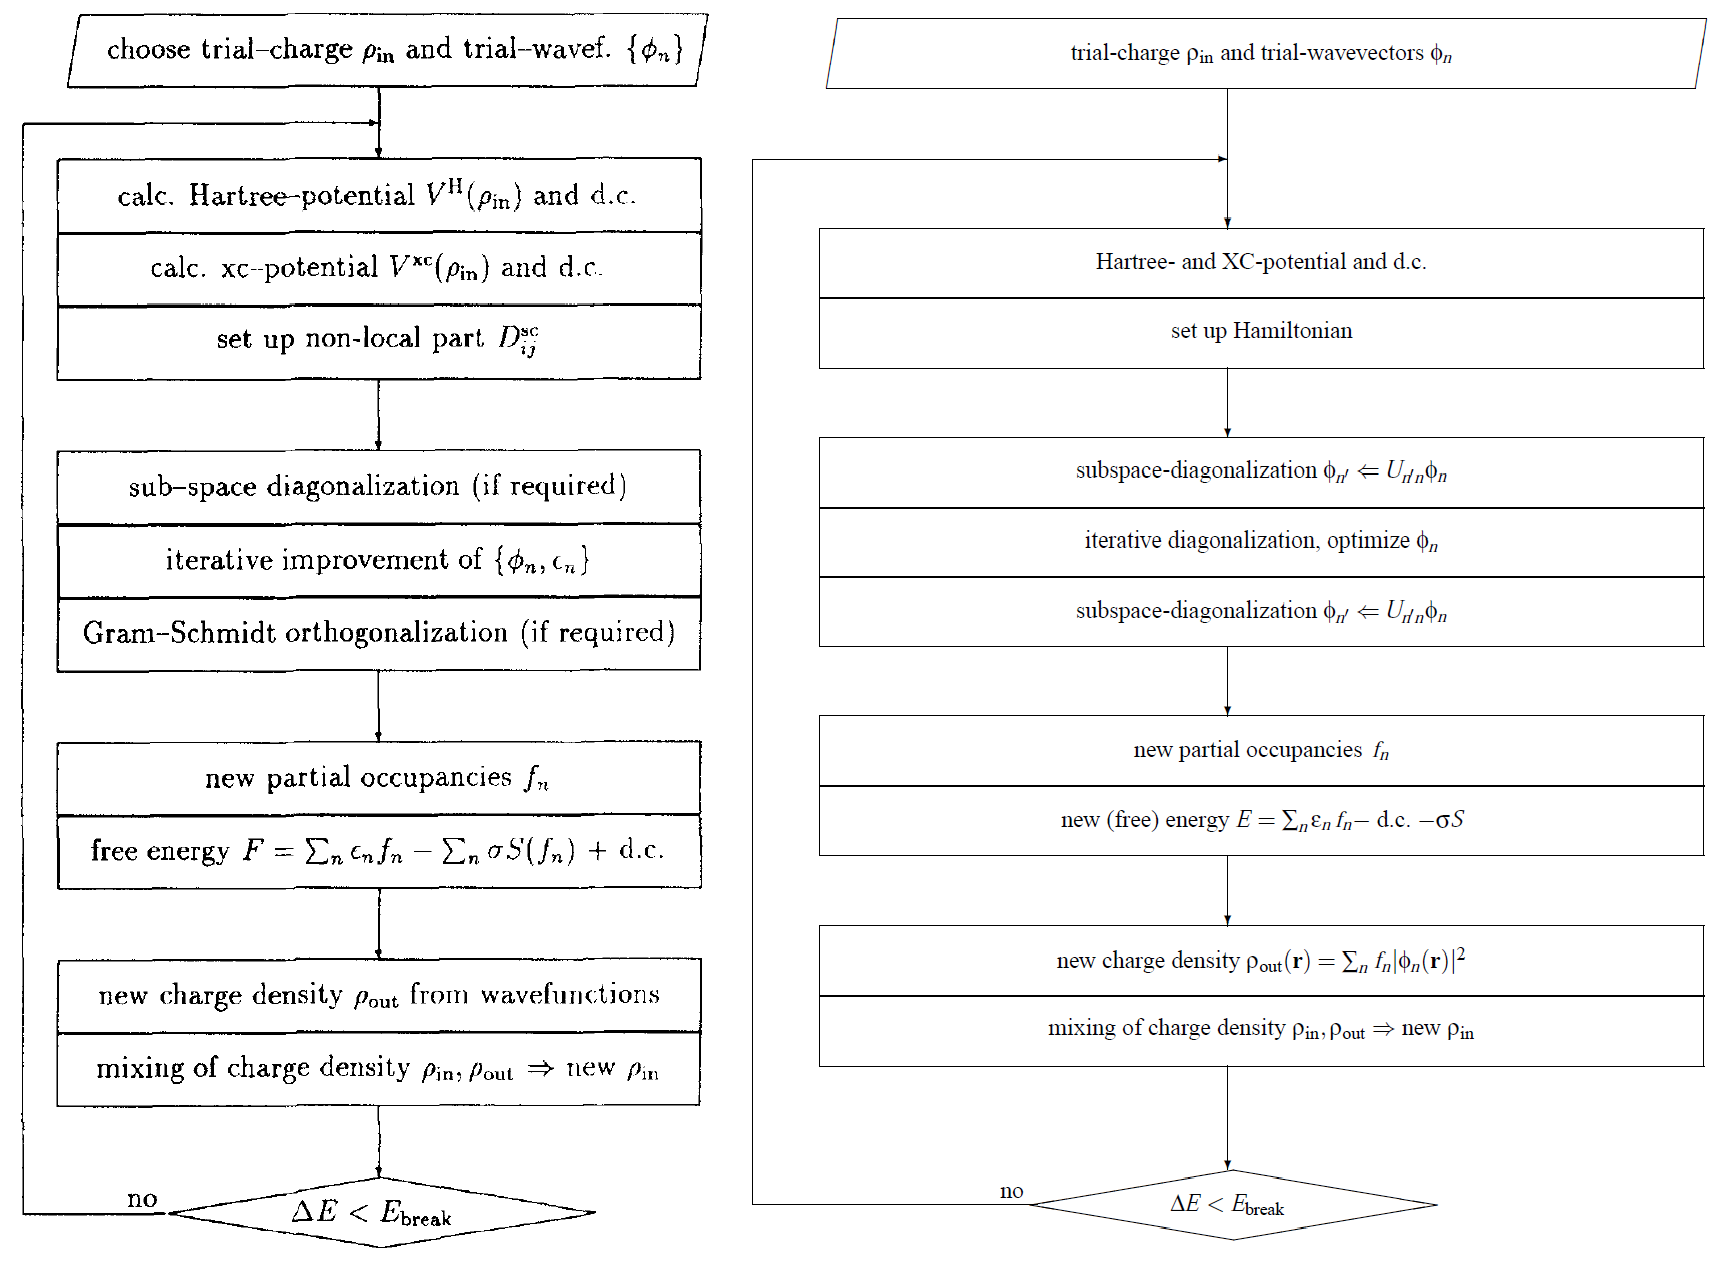
\includegraphics[height=2.7in,width=4.0in,viewport=0 0 1300 960,clip]{Figures/VASP_procedure-full.png}
%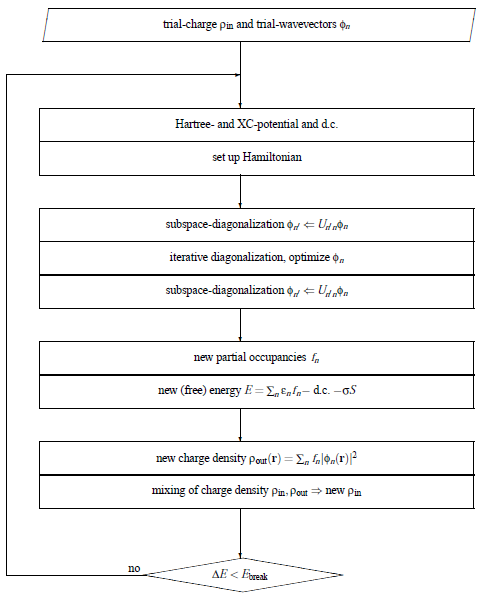
\includegraphics[height=2.1in,width=1.6in,viewport=0 0 480 630,clip]{Figures/VASP_procedure.png}
%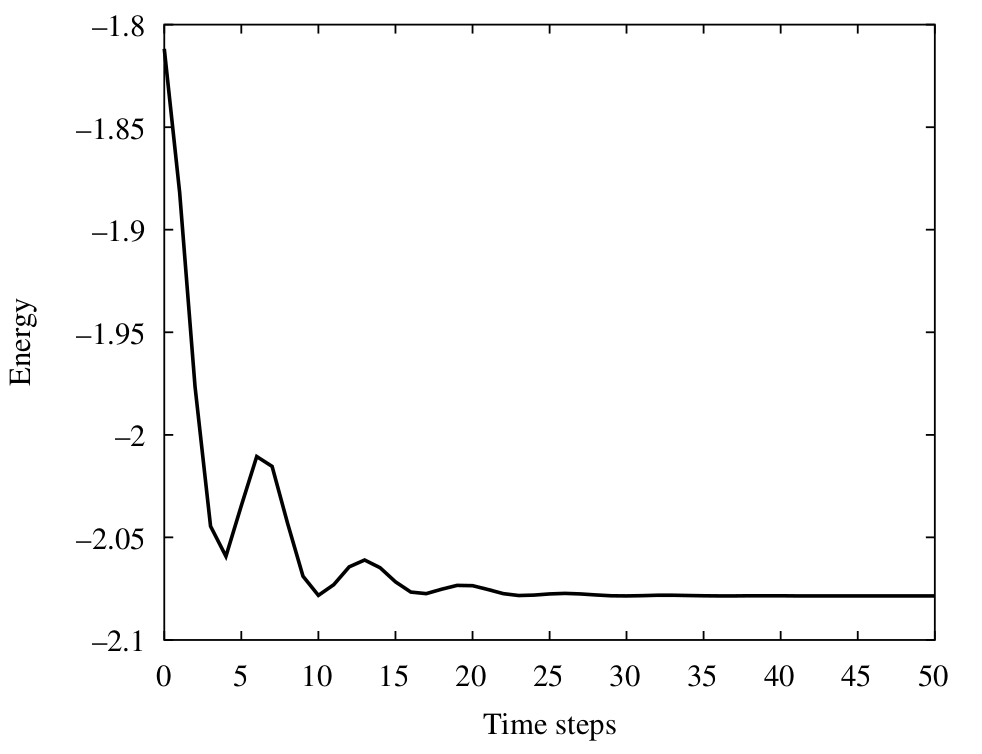
\includegraphics[height=2.1in,width=2.3in,viewport=0 0 740 600,clip]{Figures/Ab-initio-Ene.png}
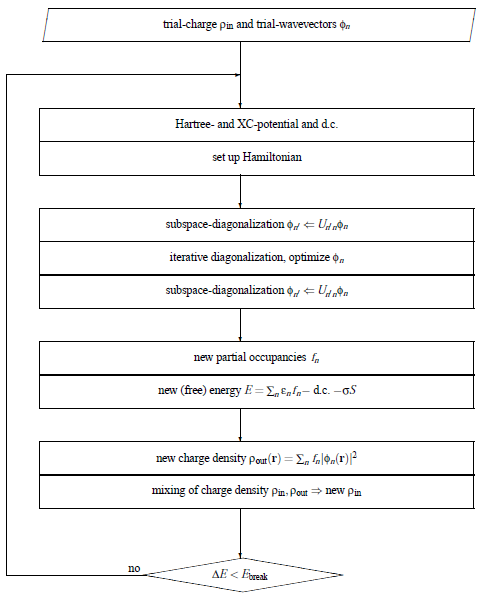
\includegraphics[height=2.75in,width=2.5in,viewport=0 0 480 630,clip]{Figures/VASP_procedure.png}
\caption{\tiny \textrm{The Flow of calculation for the KS-ground states.}}%(与文献\cite{EPJB33-47_2003}图1对比)
\label{PAW_baiseset}
\end{figure} 
}

\section{\rm{VASP}计算示例}
\subsection{{\rm Si}的电子结构:~态密度与能带}\label{Sec:Si-band}
\frame
{
	\frametitle{\textrm{Si}的结构:~\textrm{FCC}}
%{\fontsize{7.2pt}{5.2pt}\selectfont{\textrm{Si}晶胞是金刚石结构,晶胞参数$a_0=5.47\mathrm{\AA}$由结构弛豫确定}}%为了得到\textrm{Si}的电子结构,必须要完成两组连续计算:~即通过静态计算得到迭代收敛的基态电子密度,随后用获得的电子密度,按特定的对称性方向,直接计算(无需自洽迭代)得到能带。
\textrm{Si}晶胞是金刚石结构,晶胞参数$a_0=5.47\mathrm{\AA}$(由结构弛豫确定)
\vskip 5pt
\begin{figure}[h!]
\centering
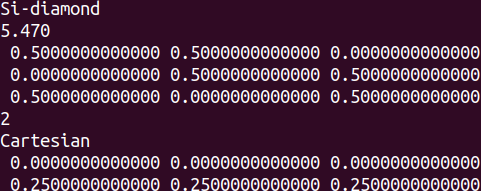
\includegraphics[height=1.6in,viewport=0 0 370 150,clip]{Figures/Si_POSCAR.png}
%\includegraphics[height=1.8in,width=4.in,viewport=30 210 570 440,clip]{PAW_projector.eps}
\caption{\fontsize{6.2pt}{5.2pt}\selectfont{\textrm{Si}的原胞:~\textrm{POSCAR}文件.}}%(与文献\cite{EPJB33-47_2003}图1对比)
\label{Si_POSCAR}
\end{figure}
}

\frame
{
	\frametitle{\textrm{Si}的初基原胞}
\vspace*{-13pt}
\begin{figure}[h!]
\centering
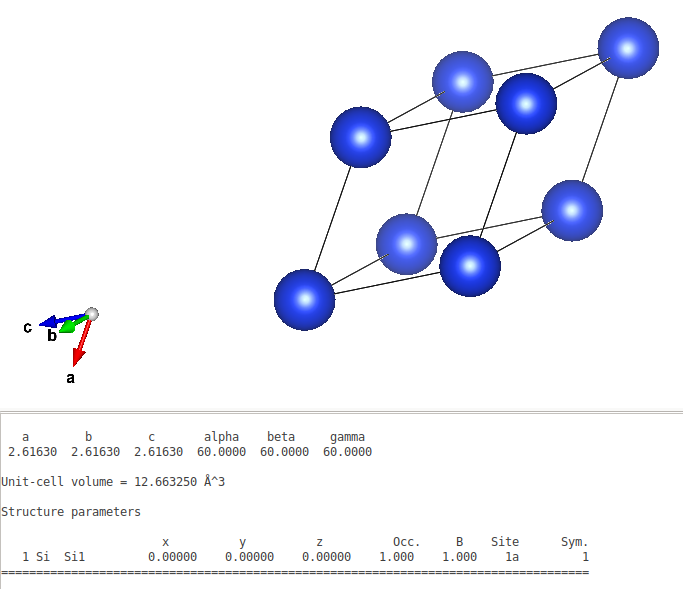
\includegraphics[height=1.78in]{Figures/VASP_example-Si_POSCAR-1-Fig.png}
\vskip 1pt
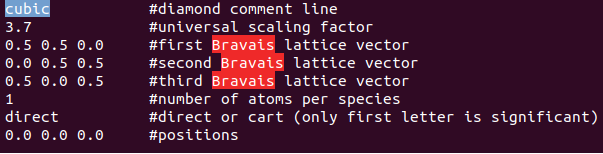
\includegraphics[height=0.98in]{Figures/VASP_example-Si_POSCAR-1.png}
%\caption{\tiny \textrm{The structure of TiC.}}%(与文献\cite{EPJB33-47_2003}图1对比)
\label{Fig:VASP-Si_POSCAR}
\end{figure}
}

\frame
{
	\frametitle{\textrm{Si}的初始计算:~输入文件}
\vspace*{-5pt}
\begin{figure}[h!]
\centering
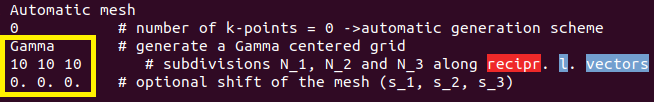
\includegraphics[height=0.62in]{Figures/VASP_example-Si_KPOINTS-G.png}
\vskip 4pt
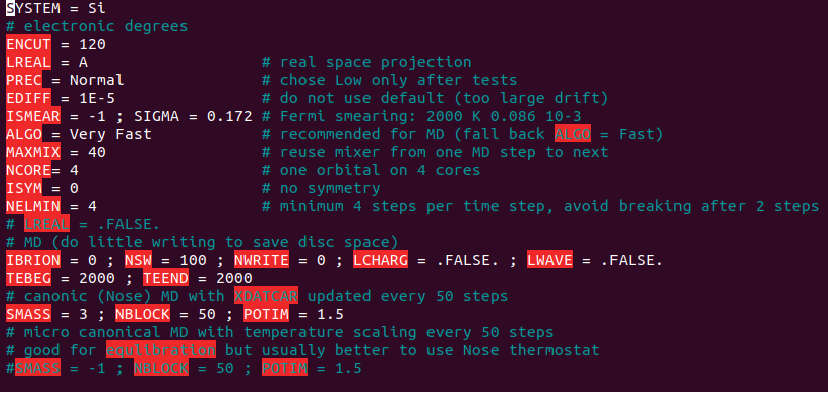
\includegraphics[height=1.88in]{Figures/VASP_example-Si_INCAR-dyn.png}
%\caption{\tiny \textrm{The structure of TiC.}}%(与文献\cite{EPJB33-47_2003}图1对比)
\label{Fig:VASP-Si_KPOINT-INCAR}
\end{figure}
}

\frame
{
	\frametitle{\textrm{Si}的初始计算:~\textrm{POTCAR}}
\vspace*{-13pt}
\begin{figure}[h!]
\centering
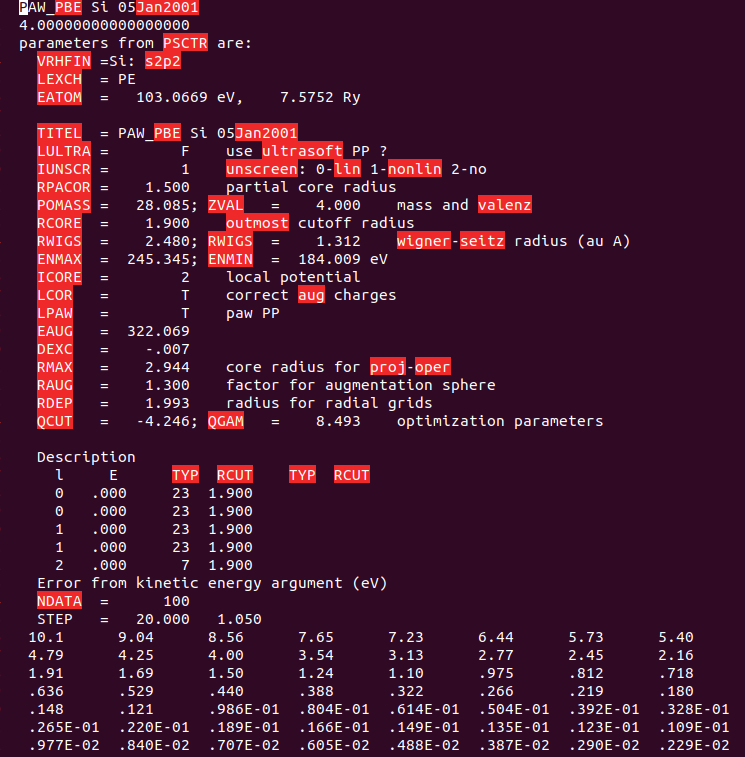
\includegraphics[height=2.88in]{Figures/VASP_example-Si_POTCAR.png}
%\caption{\tiny \textrm{The structure of TiC.}}%(与文献\cite{EPJB33-47_2003}图1对比)
\label{Fig:VASP-Si_POTCAR}
\end{figure}
}

\frame
{
	\frametitle{\textrm{VASP}计算示范:~\textrm{Si}}
\vspace*{-10pt}
\begin{figure}[h!]
\centering
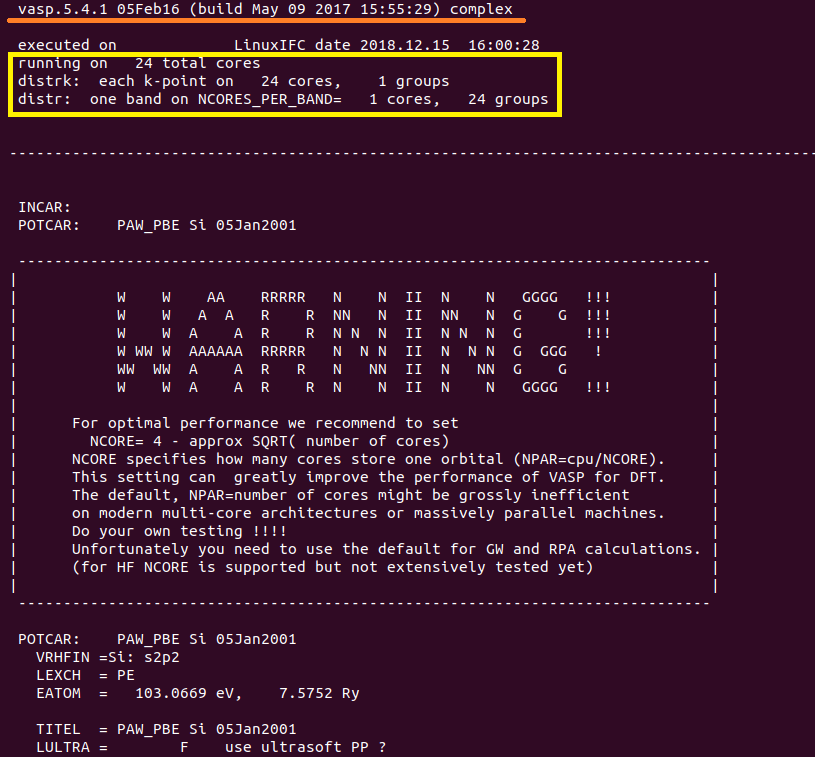
\includegraphics[width=3.0in]{Figures/VASP_example-Si_OUTCAR-1.png}
%\caption{\tiny \textrm{The structure of TiC.}}%(与文献\cite{EPJB33-47_2003}图1对比)
\label{Fig:VASP-Si_OUTCAR-part1}
\end{figure}
}

\frame
{
	\frametitle{\textrm{VASP}计算示范:~\textrm{Si}}
\vspace*{-10pt}
\begin{figure}[h!]
\centering
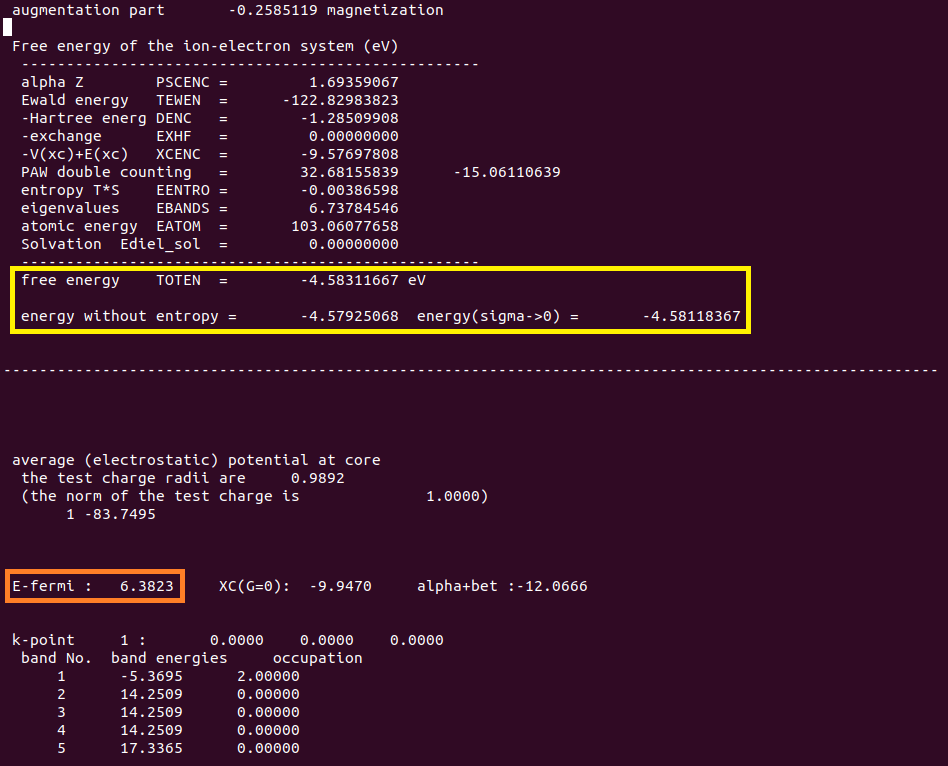
\includegraphics[width=3.5in]{Figures/VASP_example-Si_OUTCAR-2.png}
%\caption{\tiny \textrm{The structure of TiC.}}%(与文献\cite{EPJB33-47_2003}图1对比)
\label{Fig:VASP-Si_OUTCAR-part2}
\end{figure}
}

\frame
{
	\frametitle{\textrm{Si}的静态计算}
%静态计算是获得电子基态信息的重要步骤,在
静态计算:~确定基态电荷密度
\vskip 2.5pt
{\fontsize{8.5pt}{5.2pt}\selectfont{\textcolor{blue}{材料电子学性质计算的起点}}}
\vskip 3pt
{\fontsize{8.5pt}{5.2pt}\selectfont{静态计算完毕,可以从文件\textrm{OSZICAR}得到体系的基态能量,电荷密度则保存到文件\textrm{CHGCAR}中}}
%\vspace*{-10pt}
\begin{figure}[h!]
\centering
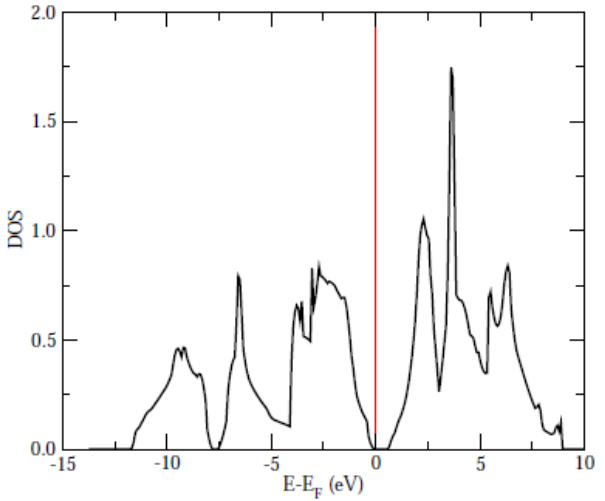
\includegraphics[width=2.5in]{Figures/VASP_cdSi_1.png}
%\caption{\tiny \textrm{The structure of TiC.}}%(与文献\cite{EPJB33-47_2003}图1对比)
\label{Fig:VASP-Si_DOS}
\end{figure}
}

%\subsection{Si的能带结构计算}
\frame
{
	\frametitle{能带计算与$\vec k$点选择}
%一般地,波矢$\vec k $的取值是三维空间(第一\textrm{Brillouin}区)中的矢量。在
	%表\ref{Tabble-kpath}给出的是\textrm{FCC}结构的第一\textrm{Brillouin}区的高对称性$\vec k$点列表。
\begin{minipage}{1.0\textwidth}
\begin{table}[!h]
\tabcolsep 0pt \vspace*{-12pt}
\fontsize{7.2pt}{5.2pt}\selectfont{
%\begin{center}
\centering
\caption{\fontsize{6.2pt}{5.2pt}\selectfont{\textrm{FCC}的第一\textrm{Brillouin}区中高对称性点的列表}}\label{Table-kpath}
\def\temptablewidth{0.95\textwidth}
\renewcommand\arraystretch{0.8} %表格宽度控制(普通表格宽度的两倍)
\rule{\temptablewidth}{1pt}
\begin{tabular*} {\temptablewidth}{@{\extracolsep{\fill}}c@{\extracolsep{\fill}}c@{\extracolsep{\fill}}c}
%-------------------------------------------------------------------------------------------------------------------------
	&\textrm{Reciprocal coordinates} &\textrm{Cartesian coordinates}\\
	\textrm{Points}	&\textrm{(unit of $b_1,b_2,b_3$)} &\textrm{unit of $2\pi/a$} \\\hline
	$\Gamma$ &0~~0~~0 &0~~0~~0 \\
	X &1/2~~0~~1/2 &0~~1~~0 \\
	W &3/4~~1/2~~1/4 &0~~1/2~~1 \\
	L &1/2~~1/2~~1/2 &1/2~~1/2~~1/2 \\
	$\Delta$ &1/4~~0~~1/4 &0~~1/2~~0 \\
	$\Lambda$ &1/ 4~~1/4~~1/4 &1/4~~1/4~~1/4 \\
\end{tabular*}
\rule{\temptablewidth}{1pt}
}
%\end{center}
\end{table}
\end{minipage}
\begin{figure}[h!]
	\vskip -8pt
\centering 
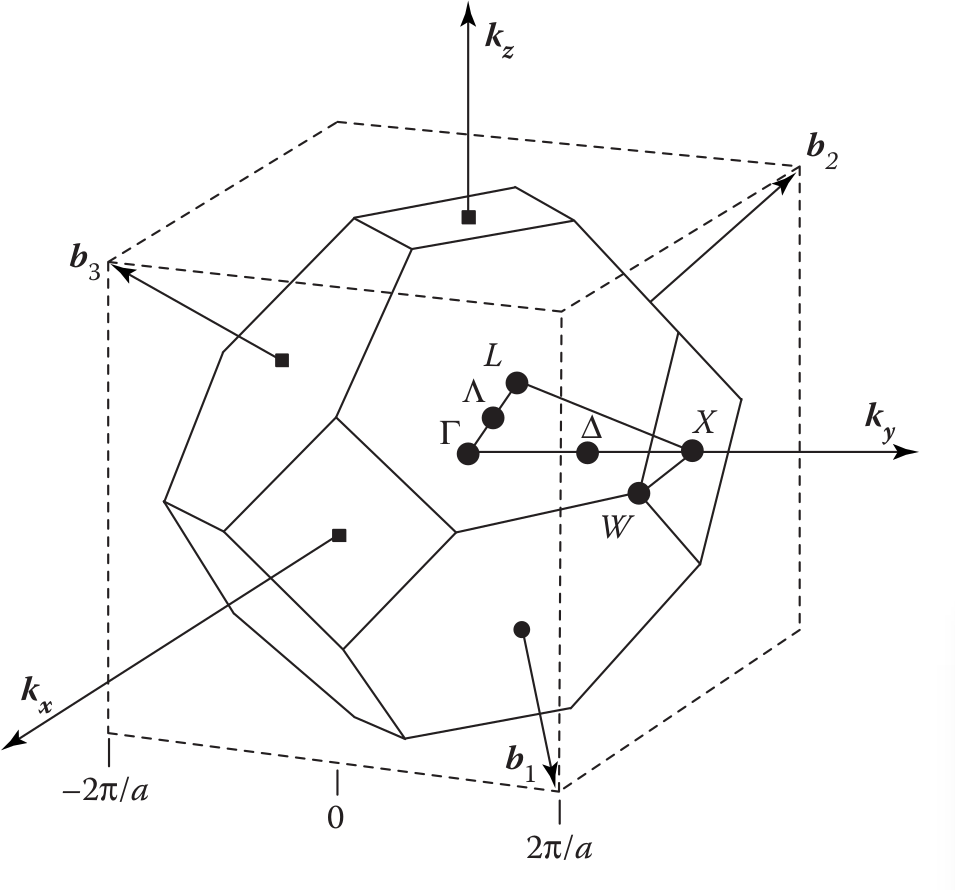
\includegraphics[height=1.7in,viewport=0 0 680 680,clip]{Figures/VASP_train-FCC-BZ.png}
%\includegraphics[height=1.8in,width=4.in,viewport=30 210 570 440,clip]{PAW_projector.eps}
\caption{\fontsize{6.2pt}{5.2pt}\selectfont{\textrm{Brillouin}区为\textrm{FCC}时的空间结构和$\vec k$-点路径关系.}}%(与文献\cite{EPJB33-47_2003}图1对比)
\label{VASP_train-FCC-BZ}
\end{figure}
	{\fontsize{7.5pt}{5.2pt}\selectfont{能带表示中的波矢$\vec k$选择:~沿不可约第一\textrm{Brillouin}区的高对称性点连线}}
%因此,为了绘制平滑的能带曲线,需要在\textrm{KPOINTS}文件中指定足够多的$\vec k$点,能带计算时,只需针对这些指定的$\vec k$点计算各轨道的能量本征值。%如图\ref{Si_KPOINTS}所示:
}

\frame
{
	\frametitle{\textrm{Si}能带计算}

%为了完成能带计算,主要是\textrm{CHGCAR}文件,其余文件改动极少。
%\subsubsection{\rm{INCAR}}%如图\ref{Si_Band-INCAR}所示。这里
%\subsubsection{\rm{KPOINTS}}
{\fontsize{7.5pt}{5.2pt}\selectfont{由\textrm{Brillouin}区$\vec k$点连线,确定\textrm{KPOINTS}文件的$\vec k$点分布:}}\\%如图所示\ref{VASP_train-FCC-BZ}。
{\fontsize{6.2pt}{5.2pt}\selectfont{沿$\vec k$点路线$\mathrm{W}-\mathrm{L}-\Gamma-\mathrm{X}-\mathrm{W}$共计80个$\vec k$点(20点/连线$\times$4组连线)}%的\textrm{KPOINTS}文件%,对应
\begin{figure}[h!]
	\vskip -5pt
\centering 
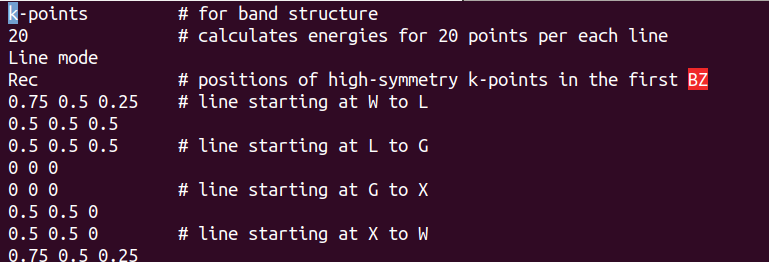
\includegraphics[width=3.6in,viewport=0 0 540 210,clip]{Figures/Si_KPOINTS.png}
%\includegraphics[height=1.8in,width=4.in,viewport=30 210 570 440,clip]{PAW_projector.eps}
\caption{\fontsize{6.2pt}{5.2pt}\selectfont{\textrm{Si}的能带计算时\textrm{KPOINTS}的设置.}}%(与文献\cite{EPJB33-47_2003}图1对比)
\label{Si_KPOINTS}
\end{figure}
%图\ref{Si_KPOINTS}给出的是\textrm{VASP}计算
}
\begin{figure}[h!] 
	\vskip -5pt
\centering
\includegraphics[height=0.5in,viewport=0 0 330 80,clip]{Figures/Si_Band-INCAR.png}
%\includegraphics[height=1.8in,width=4.in,viewport=30 210 570 440,clip]{PAW_projector.eps}
\caption{\fontsize{6.2pt}{5.2pt}\selectfont{\textrm{Si}的能带计算中的\textrm{INCAR}设置.}}%(与文献\cite{EPJB33-47_2003}图1对比)
\label{Si_Band-INCAR}
\end{figure}
{\fontsize{7.5pt}{5.2pt}\selectfont{静态计算完毕,根据能带计算需要,修改\textrm{INCAR}文件参数:~设置\textcolor{cyan}{\textit{ICHARG}}=11,电荷密度来自静态计算\textrm{CHGCAR},在计算中保持不变}}
}

\frame
{
	\frametitle{\textrm{Si}能带}
%图\ref{Si_Band-DOS}给出绘制的能带图,可见按照当前的$\vec k$点路径选择,。
\begin{figure}[h!]
	\vskip -8pt
\centering
\includegraphics[width=3.5in,viewport=0 10 920 610,clip]{Figures/Si_Band-DOS.png}
%\includegraphics[height=1.8in,width=4.in,viewport=30 210 570 440,clip]{PAW_projector.eps}
\caption{\fontsize{6.2pt}{5.2pt}\selectfont{\textrm{Si}的能带和相应的态密度图,从能带图看出\textrm{Si}是间接带隙半导体.}}%(与文献\cite{EPJB33-47_2003}图1对比)
\label{Si_Band-DOS}
\end{figure}
{\fontsize{6.2pt}{5.2pt}\selectfont{\textrm{Si}是%间接带隙
半导体,带隙$E_g=0.61\textrm{eV}$%是$\Gamma$点和$X$点之间的带隙值,同时也是图中所有$\vec k$点之间最小的能量差。
~(该值仅为实验测得带隙的$1/2$,因\textrm{DFT}先天不足,低估带隙)}}
%不过除了对带隙的低估,\textrm{DFT}计算的色散关系(能量在倒空间分布关系)是完全正确的,比如\textrm{Fermi}面附近有四个价带,四个导带,能量$\varepsilon_{\vec k}^n$随$\vec k$空间的变化逐渐改变,因此\textrm{DFT}理论的计算定性是完全正确的。实际上,其他物理量(比如波函数和电子密度),也和能量本征值有类似的倒空间分布关系。表明这样的$\vec k$点采样是合理的,能够表现物理量在不可约\textrm{Brillouin}区的定量变化。
}

%\frame
%{
%	\frametitle{\textrm{Si}的能带}
%%\vspace*{5pt}
%\begin{figure}[h!]
%\centering
%\includegraphics[width=4.0in]{Figures/VASP_cdSi_2.png}
%%\caption{\tiny \textrm{The structure of TiC.}}%(与文献\cite{EPJB33-47_2003}图1对比)
%\label{Fig:VASP-Si_Band}
%\end{figure}
%}
%
\frame
{
	\frametitle{\textrm{Si}的能带可视化:~\textrm{p4vasp}}
%\vspace*{5pt}
\begin{figure}[h!]
\centering
\includegraphics[width=4.0in]{Figures/VASP_cdSi_3.png}
%\caption{\tiny \textrm{The structure of TiC.}}%(与文献\cite{EPJB33-47_2003}图1对比)
\label{Fig:VASP-Si_p4vasp}
\end{figure}
}

%\subsubsection{\rm{能带中的本征值}}
\frame
{
	\frametitle{\textrm{Si}能带与本征值}
%因为能带计算是非自洽迭代计算,计算出来能量本征值$\varepsilon_{\vec k}^n$写入\textrm{EIGENVAL}文件中,用于绘制能带图。如图\ref{Si_Band-EIGENVAL}所示
	{\fontsize{7.2pt}{5.2pt}\selectfont{由\textrm{OUTCAR}可知\textrm{Fermi}能级为5.6980\textrm{eV}}}%)设为0~\textrm{eV},可以得到$\vec k$点和能量本征值关系的数据文件\textrm{Si-band.dat},内容如图\ref{Si_Band-data}所示
\begin{figure}[h!]
	\vskip -3pt
\centering
\includegraphics[width=4.0in,viewport=0 0 640 375,clip]{Figures/Si_Band-EIGENVAL.png}
%\includegraphics[height=1.8in,width=4.in,viewport=30 210 570 440,clip]{PAW_projector.eps}
\caption{\fontsize{6.2pt}{5.2pt}\selectfont{\textrm{VASP}计算\textrm{Si}的能量本征值文件\textrm{EIGENVAL}(部分).}}%(与文献\cite{EPJB33-47_2003}图1对比)
\label{Si_Band-EIGENVAL}
\end{figure}
%文件\textrm{EIGENVAL}中第一行是倒晶格中的$\vec k$点位置,随后8行是对应的8个能带的能量本征值:~其中前4个(\textrm{No.}~1-4)能级表示价带,是0\textrm{K}下的占据态。从\textrm{EIGENVAL}文件中提取出各$\vec k$点的能量本征值$\varepsilon_{\vec k}^n$,并将\textrm{Fermi}能级设置为0~(可以用本讲义提供的脚本\textcolor{blue}{\textrm{vasp\_to\_image.py}}实现)。运行该脚本,将\textrm{Fermi}能级(

%\begin{figure}[h!]
%\centering
%\includegraphics[height=1.2in,viewport=0 0 540 140,clip]{Si_Band-data.png}
%%\includegraphics[height=1.8in,width=4.in,viewport=30 210 570 440,clip]{PAW_projector.eps}
%\caption{\small \textrm{用于绘制\textrm{Si}能带结构的数据.}}%(与文献\cite{EPJB33-47_2003}图1对比)
%\label{Si_Band-data}
%\end{figure}
}

\section{材料模拟基础:~建模——以\rm{Materials~Studio}为例}
\frame
{
	\frametitle{\textrm{MS}的架构}
\begin{figure}[h!]
\centering
\vspace*{-0.10in}
\includegraphics[height=2.20in,width=4.15in,viewport=0 0 1275 667,clip]{Figures/MS-main_Struct.png}
\caption{\tiny \textrm{The main structure of Materials studio.}}%(与文献\cite{EPJB33-47_2003}图1对比)
\label{MS-main-structure}
\end{figure}
}

\subsection{\rm{Materials Studio}的界面框架}
\frame
{
	\frametitle{\textrm{MS}的界面框架}
\begin{figure}[h!]
\centering
\vspace*{-0.31in}
\includegraphics[height=2.45in,width=4.10in,viewport=0 0 1340 800,clip]{Figures/MS-Frame.png}
\includegraphics[height=0.45in,width=4.15in,viewport=0 0 1400 147,clip]{Figures/MS-Frame_calculators.png}
\caption{\tiny \textrm{The frame of Materials studio.}}%(与文献\cite{EPJB33-47_2003}图1对比)
\label{MS-Frame}
\end{figure}
}

%\subsection{\rm{Materials Studio:~Building}}
%\frame
%{
%	\frametitle{\textrm{MS:~Building Modules}}
%\begin{figure}[h!]
%\centering
%%\vspace*{-0.10in}
%\includegraphics[height=1.90in,width=4.10in,viewport=0 0 1259 586,clip]{Figures/MS-Building_tools.png}
%\caption{\tiny \textrm{The Building tools in Materials studio.}}%(与文献\cite{EPJB33-47_2003}图1对比)
%\label{MS-Building-tools}
%\end{figure}
%}

%\subsection{\rm{Materials Studio:~Calculator}}
%\frame
%{
%	\frametitle{\textrm{MS:~Calculator}}
%\begin{figure}[h!]
%\centering
%\vspace*{-0.15in}
%\includegraphics[height=2.75in,width=3.80in,viewport=0 0 969 728,clip]{Figures/MS-Caluculator-compare-2.png}
%\caption{\tiny \textrm{Comparing of Calculators in Materials studio.}}%(与文献\cite{EPJB33-47_2003}图1对比)
%\label{MS-Calculator-compare-2}
%\end{figure}
%}
%
%\frame
%{
%	\frametitle{\textrm{MS:~Calculator}}
%\begin{figure}[h!]
%\centering
%%\vspace*{-0.10in}
%\includegraphics[height=1.50in,width=4.10in,viewport=0 0 1517 602,clip]{Figures/MS-Caluculator-compare-1.png}
%\caption{\tiny \textrm{Calculators in Materials studio:~parameters.}}%(与文献\cite{EPJB33-47_2003}图1对比)
%\label{MS-Calculator-compare-1}
%\end{figure}
%}
%
%\frame
%{
%	\frametitle{\textrm{MS:~XC-functionals}}
%\begin{figure}[h!]
%\centering
%\vspace*{-0.10in}
%\includegraphics[height=2.50in,width=4.10in,viewport=0 0 1261 752,clip]{Figures/MS-xc_functional-compare.png}
%\caption{\tiny \textrm{XC-functionals in Materials studio.}}%(与文献\cite{EPJB33-47_2003}图1对比)
%\label{MS-xc_functional-compare}
%\end{figure}
%}
%
\frame
{
	\frametitle{\textrm{MS}的界面框架:~\textrm{Indigo}}
\begin{figure}[h!]
\centering
\vspace*{-0.28in}
\includegraphics[height=2.85in,width=4.15in,viewport=0 0 1140 800,clip]{Figures/MS-Frame_example.png}
\caption{\tiny \textrm{The frame of Materials studio:~Example Indigo.}}%(与文献\cite{EPJB33-47_2003}图1对比)
\label{MS-Frame_example}
\end{figure}
}

\subsection{\rm{Materials Studio:~Quick Start}}
\frame
{
	\frametitle{\textrm{MS:~Quick Start-01}}
\begin{figure}[h!]
\centering
\vspace*{-0.21in}
\includegraphics[height=2.70in,width=4.10in,viewport=0 0 1134 740,clip]{Figures/MS-New_Project-01.png}
\caption{\tiny \textrm{Quick Start for Materials studio:~Step-01.}}%(与文献\cite{EPJB33-47_2003}图1对比)
\label{MS-Quick_Start-01}
\end{figure}
}

\frame
{
	\frametitle{\textrm{MS:~Quick Start-02}}
\begin{figure}[h!]
\centering
\vspace*{-0.10in}
\includegraphics[height=2.70in,width=4.00in,viewport=0 0 1045 776,clip]{Figures/MS-New_Project-02.png}
\caption{\tiny \textrm{Quick Start for Materials studio:~Step-02.}}%(与文献\cite{EPJB33-47_2003}图1对比)
\label{MS-Quick_Start-02}
\end{figure}
}

\frame
{
	\frametitle{\textrm{MS:~Quick Start-03}}
\begin{figure}[h!]
\centering
\vspace*{-0.10in}
\includegraphics[height=2.68in,width=4.00in,viewport=0 0 1090 760,clip]{Figures/MS-New_Project-03.png}
\caption{\tiny \textrm{Quick Start for Materials studio:~Step-03.}}%(与文献\cite{EPJB33-47_2003}图1对比)
\label{MS-Quick_Start-03}
\end{figure}
}

%\subsection{\rm{Materials Studio:~Modelling}}
\frame
{
	\frametitle{\textrm{MS:~Quick Start-Modelling-01}}
\begin{figure}[h!]
\centering
\vspace*{-0.10in}
\includegraphics[height=2.60in,width=4.00in,viewport=0 0 1090 710,clip]{Figures/MS-New_Project-04.png}
\caption{\tiny \textrm{Quick Start for Materials studio:~Modelling-01.}}%(与文献\cite{EPJB33-47_2003}图1对比)
\label{MS-Quick_Start-Modelling-01}
\end{figure}
}

\frame
{
	\frametitle{\textrm{MS:~Quick Start-Modelling-02}}
\begin{figure}[h!]
\centering
\vspace*{-0.10in}
\includegraphics[height=2.68in,width=4.00in,viewport=0 0 1090 760,clip]{Figures/MS-New_Project-05.png}
\caption{\tiny \textrm{Quick Start for Materials studio:~Modelling-02.}}%(与文献\cite{EPJB33-47_2003}图1对比)
\label{MS-Quick_Start-Modelling-02}
\end{figure}
}

\frame
{
	\frametitle{\textrm{MS:~Modelling Crystal-01}}
\begin{figure}[h!]
\centering
\vspace*{-0.10in}
\includegraphics[height=2.68in,width=4.00in,viewport=0 0 1090 760,clip]{Figures/MS-New_Project-06.png}
\caption{\tiny \textrm{Modelling crystal by Materials studio.}}%(与文献\cite{EPJB33-47_2003}图1对比)
\label{MS-Modelling-Crystal-01}
\end{figure}
}

\frame
{
	\frametitle{\textrm{MS:~Modelling Crystal-02}}
\begin{figure}[h!]
\centering
\vspace*{-0.15in}
\includegraphics[height=2.75in,width=4.00in,viewport=0 0 1090 814,clip]{Figures/MS-New_Project-07.png}
\caption{\tiny \textrm{Modelling crystal by Materials studio:~Parameters.}}%(与文献\cite{EPJB33-47_2003}图1对比)
\label{MS-Modelling-Crystal-02}
\end{figure}
}

\frame
{
	\frametitle{\textrm{MS:~Modelling Crystal-03}}
\begin{figure}[h!]
\centering
\vspace*{-0.15in}
\includegraphics[height=2.75in,width=3.70in,viewport=0 0 818 616,clip]{Figures/MS-New_Project-08.png}
\caption{\tiny \textrm{Modelling crystal by Materials studio:~Lattice-parameters.}}%(与文献\cite{EPJB33-47_2003}图1对比)
\label{MS-Modelling-Crystal-03}
\end{figure}
}

\frame
{
	\frametitle{\textrm{MS:~Modelling Crystal-04}}
\begin{figure}[h!]
\centering
\vspace*{-0.10in}
\includegraphics[height=2.70in,width=4.00in,viewport=0 0 1090 759,clip]{Figures/MS-New_Project-09.png}
\caption{\tiny \textrm{Modelling crystal by Materials studio:~Elements.}}%(与文献\cite{EPJB33-47_2003}图1对比)
\label{MS-Modelling-Crystal-04}
\end{figure}
}

\frame
{
	\frametitle{\textrm{MS:~Modelling Crystal example:~Si}}
\begin{figure}[h!]
\centering
\vspace*{-0.10in}
\includegraphics[height=2.70in,width=2.30in,viewport=0 0 546 747,clip]{Figures/MS-New_Project-10-Si_example.png}
\caption{\tiny \textrm{Modelling crystal by Materials studio:~Si.}}%(与文献\cite{EPJB33-47_2003}图1对比)
\label{MS-Modelling-Crystal-05}
\end{figure}
}

\frame
{
	\frametitle{\textrm{MS:~Modelling Crystal example:~Si}}
\begin{figure}[h!]
\centering
\vspace*{-0.10in}
\includegraphics[height=2.65in,width=4.00in,viewport=0 0 1090 698,clip]{Figures/MS-New_Project-11-Si_crystal.png}
\caption{\tiny \textrm{Modelling crystal by Materials studio:~Si.}}%(与文献\cite{EPJB33-47_2003}图1对比)
\label{MS-Modelling-Crystal-06}
\end{figure}
}

\subsection{\rm{Materials Studio:~Calculation}}
\frame
{
	\frametitle{\textrm{MS:~CASTEP Calculation example:~Si}}
\begin{figure}[h!]
\centering
\vspace*{-0.10in}
\includegraphics[height=2.62in,width=4.00in,viewport=0 0 1210 740,clip]{Figures/MS-CASTEP-01-Si.png}
\caption{\tiny \textrm{CASTEP Calculation by Materials studio:~Si.}}%(与文献\cite{EPJB33-47_2003}图1对比)
\label{MS-CASTEP-Calculation-01}
\end{figure}
}

\frame
{
	\frametitle{\textrm{MS:~CASTEP Calculation example:~Si}}
\begin{figure}[h!]
\centering
%\vspace*{-0.10in}
\includegraphics[height=2.05in,width=1.95in,viewport=0 0 756 787,clip]{Figures/MS-CASTEP-02-Si-parameter-1.png}
\includegraphics[height=2.05in,width=1.95in,viewport=0 0 775 798,clip]{Figures/MS-CASTEP-02-Si-parameter-2.png}
\caption{\tiny \textrm{CASTEP Calculation by Materials studio:~Parameter.}}%(与文献\cite{EPJB33-47_2003}图1对比)
\label{MS-CASTEP-Calculation-02}
\end{figure}
}

\frame
{
	\frametitle{\textrm{MS:~CASTEP Calculation example:~Si}}
\begin{figure}[h!]
\centering
\vspace*{-0.10in}
\includegraphics[height=2.15in,width=1.95in,viewport=0 -50 650 700,clip]{Figures/MS-CASTEP-13-Si-Calculat-Electron-step.png}
\includegraphics[height=2.15in,width=1.95in,viewport=0 0 636 774,clip]{Figures/MS-CASTEP-13-Si-Calculat-Electron-detail.png}
\caption{\tiny \textrm{CASTEP Calculation by Materials studio:~Electron-step.}}%(与文献\cite{EPJB33-47_2003}图1对比)
\label{MS-CASTEP-Calculation-electron}
\end{figure}
}

\frame
{
	\frametitle{\textrm{MS:~CASTEP Calculation example:~Si}}
\begin{figure}[h!]
\centering
%\vspace*{-0.10in}
\includegraphics[height=1.15in,width=3.30in,viewport=0 0 1070 452,clip]{Figures/MS-CASTEP-03-Si-input-1.png}
\includegraphics[height=1.15in,width=4.00in,viewport=0 0 1070 355,clip]{Figures/MS-CASTEP-03-Si-input-2.png}
\caption{\tiny \textrm{CASTEP Calculation.}}%(与文献\cite{EPJB33-47_2003}图1对比)
\label{MS-CASTEP-Calculation-03}
\end{figure}
}

\frame
{
	\frametitle{\textrm{MS:~CASTEP Calculation example:~Si}}
\begin{figure}[h!]
\centering
\vspace*{-0.10in}
\includegraphics[height=2.65in,width=2.63in,viewport=0 0 643 698,clip]{Figures/MS-CASTEP-04-Si-sever.png}
\caption{\tiny \textrm{CASTEP Calculation by Materials studio:~Connect to localhost.}}%(与文献\cite{EPJB33-47_2003}图1对比)
\label{MS-CASTEP-Calculation-sever}
\end{figure}
}

\frame
{
	\frametitle{\textrm{MS:~CASTEP Calculation example:~Si}}
\begin{figure}[h!]
\centering
\vspace*{-0.10in}
\includegraphics[height=2.60in,width=4.00in,viewport=0 0 1210 740,clip]{Figures/MS-CASTEP-05-Si-Calculat.png}
\caption{\tiny \textrm{CASTEP Calculation by Materials studio:~Run.}}%(与文献\cite{EPJB33-47_2003}图1对比)
\label{MS-CASTEP-Calculation-Run}
\end{figure}
}

\frame
{
	\frametitle{\textrm{MS:~CASTEP Calculation example:~Si}}
\begin{figure}[h!]
\centering
%\vspace*{-0.10in}
\includegraphics[height=1.50in,width=4.00in,viewport=0 0 1070 469,clip]{Figures/MS-CASTEP-06-Si-Calculat-finish.png}
\caption{\tiny \textrm{CASTEP Calculation by Materials studio:~Complete.}}%(与文献\cite{EPJB33-47_2003}图1对比)
\label{MS-CASTEP-Calculation-Complete}
\end{figure}
}

\frame
{
	\frametitle{\textrm{MS:~CASTEP Calculation example:~Si}}
\begin{figure}[h!]
\centering
\vspace*{-0.10in}
\includegraphics[height=2.66in,width=4.00in,viewport=0 0 1150 801,clip]{Figures/MS-CASTEP-07-Si-Calculat-data.png}
\caption{\tiny \textrm{CASTEP Calculation by Materials studio:~Finish.}}%(与文献\cite{EPJB33-47_2003}图1对比)
\label{MS-CASTEP-Calculation-data}
\end{figure}
}

\frame
{
	\frametitle{\textrm{MS:~CASTEP Calculation example:~Si}}
\begin{figure}[h!]
\centering
\vspace*{-0.10in}
\includegraphics[height=2.60in,width=4.00in,viewport=0 0 1039 790,clip]{Figures/MS-CASTEP-08-Si-Calculat-SCF.png}
\caption{\tiny \textrm{CASTEP Calculation by Materials studio:~SCF.}}%(与文献\cite{EPJB33-47_2003}图1对比)
\label{MS-CASTEP-Calculation-SCF}
\end{figure}
}

\frame
{
	\frametitle{\textrm{MS:~CASTEP Analysis example:~Si}}
\begin{figure}[h!]
\centering
\vspace*{-0.10in}
\includegraphics[height=2.60in,width=4.00in,viewport=0 0 1210 742,clip]{Figures/MS-CASTEP-09-Si-Analysis.png}
\caption{\tiny \textrm{CASTEP Analysis by Materials studio.}}%(与文献\cite{EPJB33-47_2003}图1对比)
\label{MS-CASTEP-Analysis}
\end{figure}
}

\frame
{
	\frametitle{\textrm{MS:~CASTEP Analysis example:~Si}}
\begin{figure}[h!]
\centering
\vspace*{-0.10in}
\includegraphics[height=2.66in,width=2.30in,viewport=0 0 567 813,clip]{Figures/MS-CASTEP-10-Si-Analysis-parameter.png}
\caption{\tiny \textrm{CASTEP Analysis by Materials studio:~Parameter.}}%(与文献\cite{EPJB33-47_2003}图1对比)
\label{MS-CASTEP-Analysis-parameter}
\end{figure}
}

\frame
{
	\frametitle{\textrm{MS:~CASTEP Analysis example:~Si}}
\begin{figure}[h!]
\centering
\vspace*{-0.10in}
\includegraphics[height=2.60in,width=4.00in,viewport=0 0 1210 742,clip]{Figures/MS-CASTEP-11-Si-Analysis-charge.png}
\caption{\tiny \textrm{CASTEP Analysis by Materials studio:~Charge.}}%(与文献\cite{EPJB33-47_2003}图1对比)
\label{MS-CASTEP-Analysis-Charge}
\end{figure}
}

\frame
{
	\frametitle{\textrm{MS:~CASTEP Analysis example:~Si}}
\begin{figure}[h!]
\centering
\vspace*{-0.10in}
\includegraphics[height=2.60in,width=4.00in,viewport=0 0 1210 742,clip]{Figures/MS-CASTEP-11-Si-Analysis-display.png}
\caption{\tiny \textrm{CASTEP Analysis by Materials studio:~Display-style.}}%(与文献\cite{EPJB33-47_2003}图1对比)
\label{MS-CASTEP-Analysis-display}
\end{figure}
}

\frame
{
	\frametitle{\textrm{MS:~CASTEP Analysis example:~Si}}
\begin{figure}[h!]
\centering
%\vspace*{-0.10in}
\includegraphics[height=2.00in,width=1.95in,viewport=0 0 810 820,clip]{Figures/MS-CASTEP-12-Si-Analysis-display-parameter-1.png}
\includegraphics[height=2.00in,width=1.95in,viewport=0 0 802 822,clip]{Figures/MS-CASTEP-12-Si-Analysis-display-parameter-2.png}
\caption{\tiny \textrm{CASTEP Analysis by Materials studio:~Display-parameter.}}%(与文献\cite{EPJB33-47_2003}图1对比)
\label{MS-CASTEP-Analysis-display-parameter}
\end{figure}
}

\appendix
\frame
{
	\frametitle{\rm{DFT}之歌}
\begin{figure}[h!]
	\vspace{-10pt}
\centering
\includegraphics[height=2.85in,width=3.8in,viewport=0 350 550 720,clip]{Figures/DFT_song-1.pdf}
%\caption{\tiny \textrm{The Nolbel Prize in Chemistry 1998 Summary.}}%(与文献\cite{EPJB33-47_2003}图1对比)
\label{DFT_Song_01}
\end{figure}
}

\frame
{
	\frametitle{}
\begin{figure}[h!]
	\vspace{-10pt}
\centering
\includegraphics[height=1.95in,width=3.8in,viewport=0 80 550 352,clip]{Figures/DFT_song-1.pdf}
\includegraphics[height=0.70in,width=3.8in,viewport=0 650 550 750,clip]{Figures/DFT_song-2.pdf}
%\caption{\tiny \textrm{The Nolbel Prize in Chemistry 1998 Summary.}}%(与文献\cite{EPJB33-47_2003}图1对比)
\label{DFT_Song_02}
\end{figure}
}

\frame
{
	\frametitle{}
\begin{figure}[h!]
	\vspace{-10pt}
\centering
\includegraphics[height=2.10in,width=3.8in,viewport=0 350 550 650,clip]{Figures/DFT_song-2.pdf}
%\caption{\tiny \textrm{The Nolbel Prize in Chemistry 1998 Summary.}}%(与文献\cite{EPJB33-47_2003}图1对比)
\includemovie[poster, controls, mouse, url] {0.8\textwidth}{0.1\textwidth}{Figures/DFT_Song.mp3}     %
%\includemovie[poster, controls, mouse, url] {0.8\textwidth}{0.2\textwidth}{Figures/DFT_Song_accompany.mp3}     %
\label{DFT_Song_03}
\end{figure}
}
